%Chapter 6 will look at the results from the experiments and how the performance of the new software defined radiometer measured up.

%Chapter 6: Results and Analysis

%Intro paragraph.
%Experiment 1
%	Data collected.
%	Analysis of data: Interpret the data, what was learned from the data
%Experiment 2
%	Data collected.
%	Analysis of data: Interpret the data, what was learned from the data
%Experiment X
%	Data collected.
%	Analysis of data: Interpret the data, what was learned from the data
%Price/Weight/Quality analysis (Traditional Radiometer vs. Software Defined Radiometer)
%Summary paragraph, the summary paragraph the summarized the analysis of the results.

\chapter{RESULTS AND ANALYSIS}\label{ch:results}
This chapter presents the results obtained from the experiments outlined in Chapter \ref{ch:exp_design}.  We discuss the analysis of the results and what was learned from each experiment.  This chapter concludes with a trade off analysis between SDR-based radiometer and a traditional radiometer in terms of cost and weight.

\section{Experiment I - Software Defined Radio Based Radiometer Verification and Calibration} \label{Exp1_results}
As outlined in Chapter \ref{ch:exp_design}, Section \ref{Exp1}, this experiment verifies the operation of a software defined radio based radiometer.  This is done by performing experiments that are similar to the verification and calibration methods used for a traditional radiometer.  We compare our results to those of a square-law detector receiving the same signal.

\subsection{Data Collected}\label{Exp1_data}

For this experiment, total power measurements were collected from the software defined radio based radiometer and the square-law detector.  This data is then calibrated using the known physical temperature of the matched load.  Table \ref{exp1_datapoints} shows the values collected during the experiment and is used to calibrate the raw total power measurements.

\begin{table}[h!tb] \centering
\isucaption{Total Power calibration data points}
\label{exp1_datapoints}
% Use: \begin{tabular{|lcc|} to put table in a box
\begin{tabular}{lcc} \hline
\textbf{rQ Value} & \textbf{$X^2$ Voltage (V)} & \textbf{Temperature (K)} \\ \hline
.1139 & 1.9846 & 77 \\
.1730 & 2.1065 & 271.65 \\ \hline
\end{tabular}
\end{table}

\subsection{Data Analysis}\label{Exp1_analysis}

To analyze the results, iPython Notebook is used to read our data and generate the graphs used in this thesis.  This tool uses Python along with HTML and Markdown code to generate a virtual notebook for each experiment.  

\emph{Software Defined Radio Data.}  The SDR records the total power measurements in a binary file that either Matlab or Python can read.  This file format is explained in section \ref{exp1_data}.  We begin by looking at the raw or uncalibrated total power readings.  This power information is information collected after the total power radio block in GNURadio and is explained in Chapter \ref{ch:implementation}.  Because the values are uncalibrated total power readings, there are no units.

\begin{figure}[h!tb] \centering
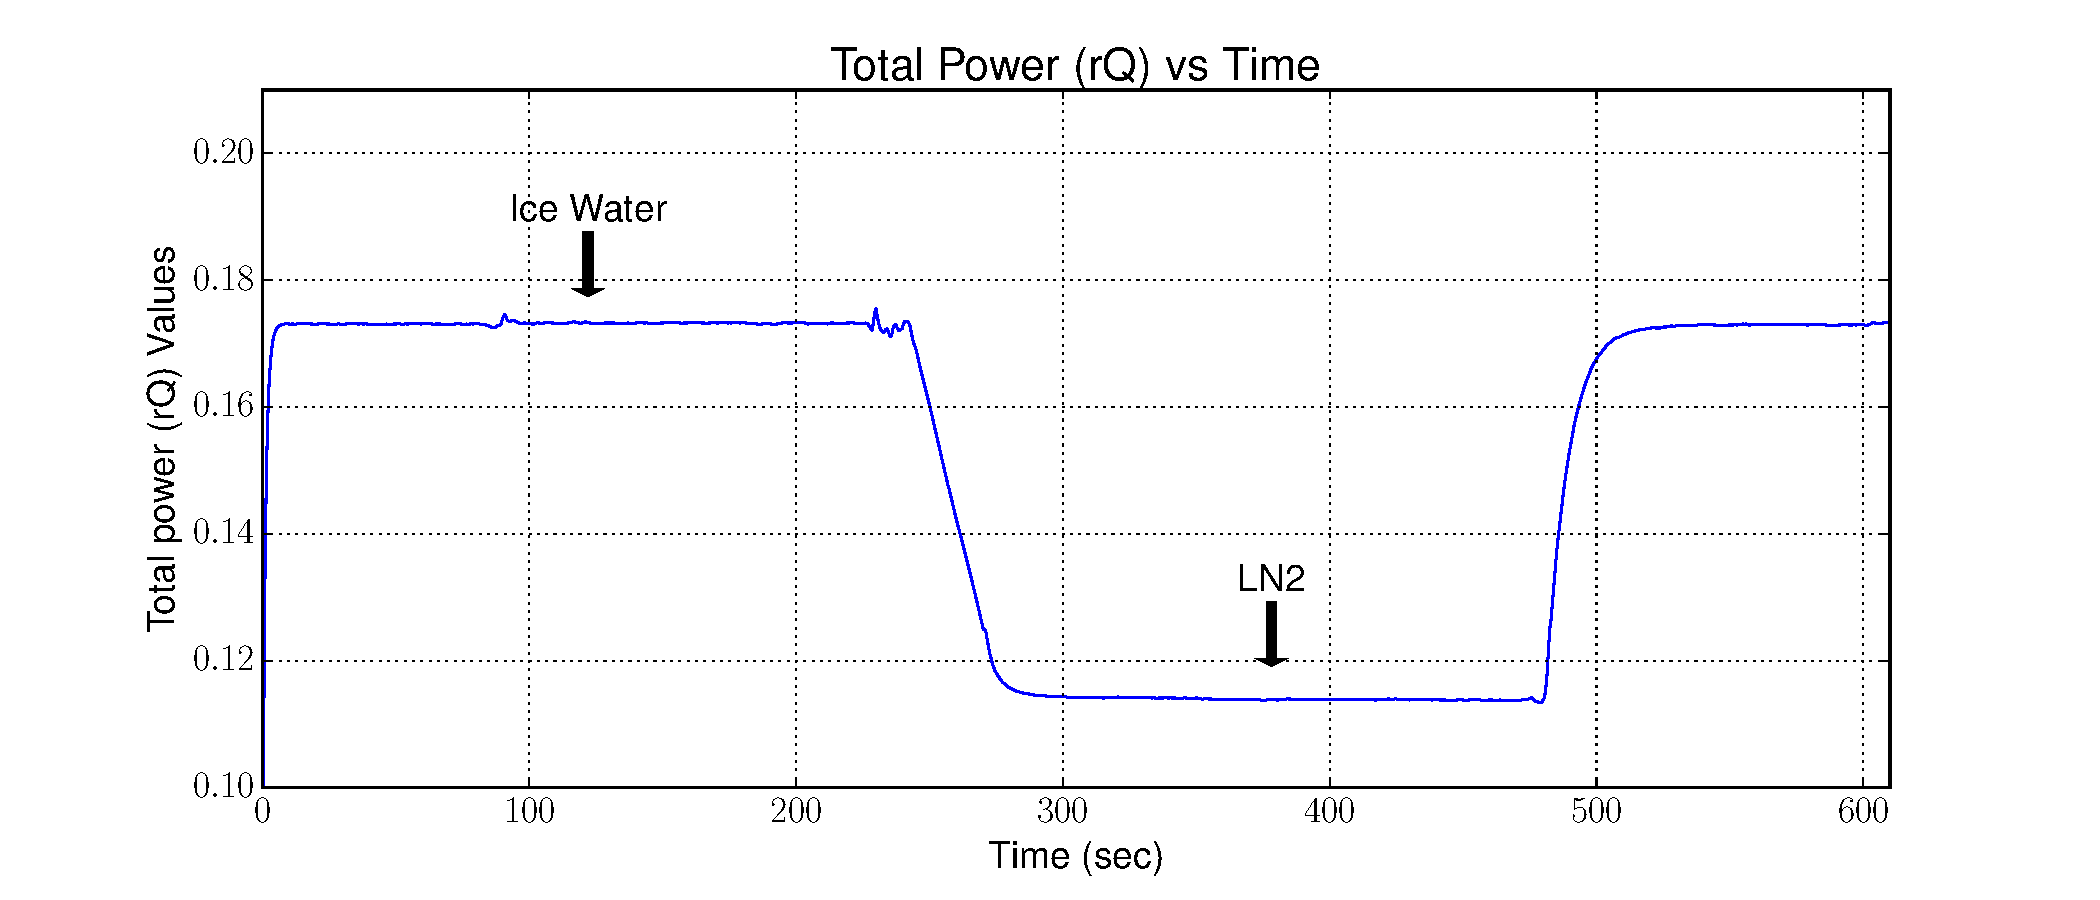
\includegraphics[width=\textwidth]{Experiments/Exp1/rqvstime_annotate.pdf}
\isucaption{Graph of the uncalibrated SDR total power values of Experiment I}
\label{SDR_rQ}
\end{figure}

Figure \ref{SDR_rQ} shows the total power reading versus time.  Figure \ref{SDR_rQ} has been annotated to show which medium the matched load has been placed in (i.e. Ice water and LN2).  Since we know the temperatures of the ice water and LN2, we can calibrate these readings to a noise temperature reading.  This is done by reading a calibration file we have stored in a csv format and solving for the slope of a line.  This was accomplished using the following code written in Python.

\lstset{language=Python}
\begin{lstlisting}[frame=single,keywordstyle=\color{blue}]
a=numpy.array([[rQ_values[0],1.0],[rQ_values[1],1.0]],numpy.float32)
b=numpy.array([temp_values[0],temp_values[1]])
z=numpy.linalg.solve(a,b)
\end{lstlisting}

Now that we have our calibration points, we can re-graph this data as calibrated noise temperature as shown in Figure \ref{SDR_Calibrated}.  Figure \ref{SDR_Calibrated} is also colorized to represent ``warmer'' to ``cooler'' noise temperatures.

\begin{figure}[h!tb] \centering

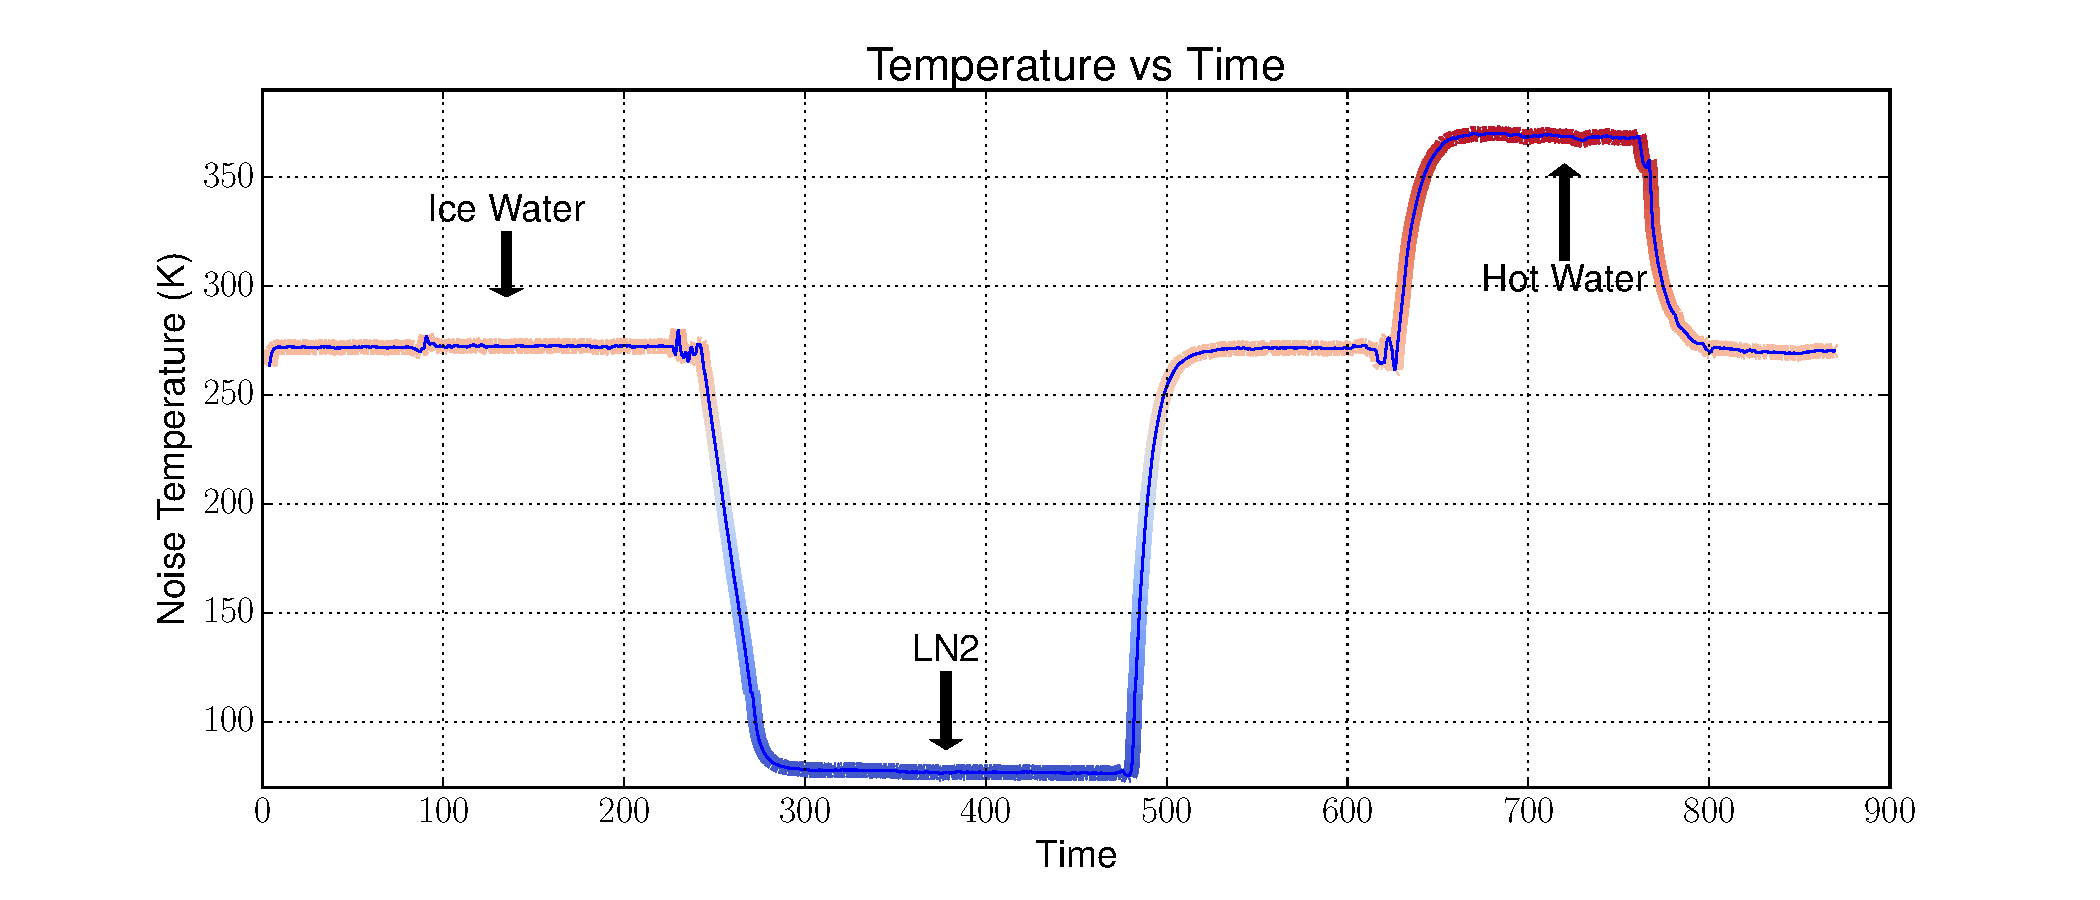
\includegraphics[width=\textwidth]{Experiments/Exp1/sdr_calibrated_color.pdf}

\isucaption{Graph of the SDR calibrated noise temperature for Experiment I}
\label{SDR_Calibrated}
\end{figure}

\emph{Square Law Detector Data.}  Now that we have looked at the software defined radio data, we want to examine the square-law detector data and then compare the two.  The square-law detector gives us power information as a voltage.  In order to compare the square-law detector to the SDR data we will also calibrate it as a noise temperature.  We can do that using the same method as the SDR and calibrate the voltages to the known temperature references.  It can be see in Figure \ref{X2_Raw} that the data from the square-law detector is very noisy.  Therefore, we use a filter to smooth out the data.

\begin{figure}[h!tb] \centering
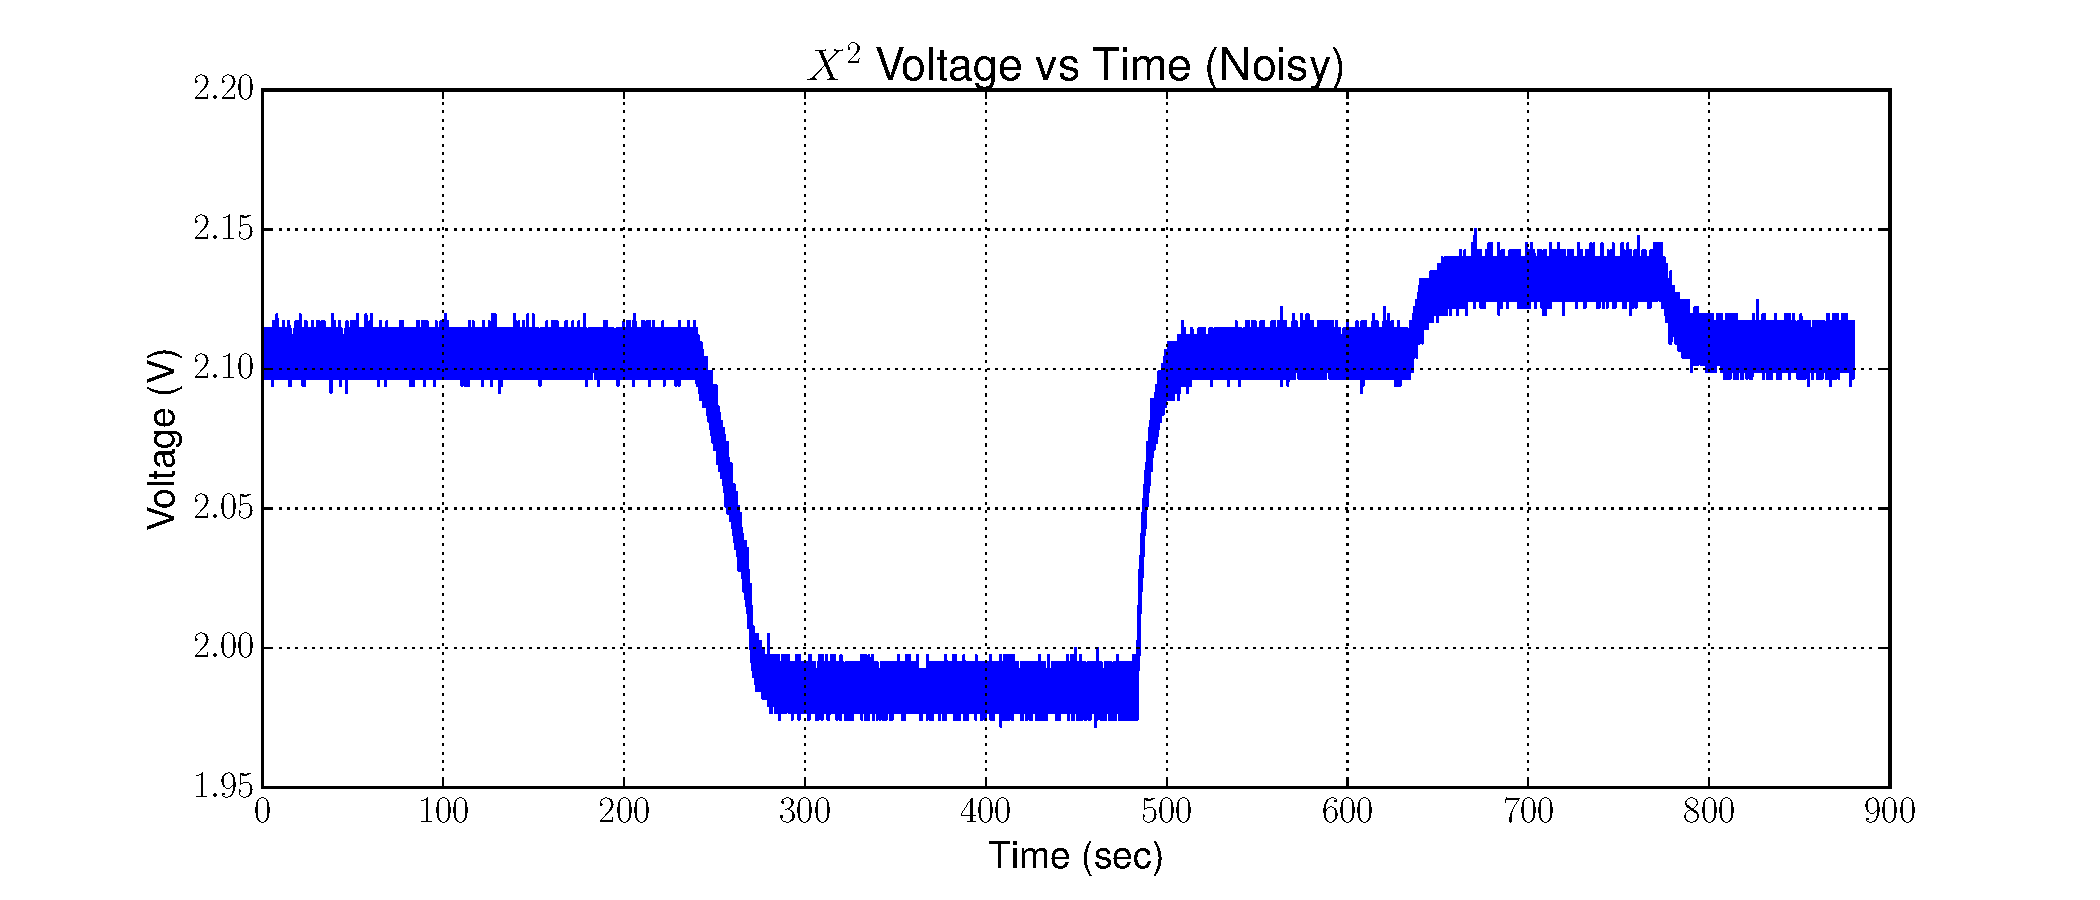
\includegraphics[width=\textwidth]{Experiments/Exp1/noisy_voltage.pdf}
\isucaption{Unfiltered data from the square-law detector collected in Experiment I}
\label{X2_Raw}
\end{figure}

To filter the data, Python in conjunction with SciPy is used.  For this experiment, we use a low pass filter to smooth out the signal.  The following code applies the filter to the data.

\begin{lstlisting}[frame=single,keywordstyle=\color{blue}]
from scipy import signal
N=100  # Number of taps
Fc=40  # Cutoff Frequency
Fs=1600  #Sample Frequency
h=scipy.signal.firwin(numtaps=N, cutoff=Fc, nyq=Fs/2)
x2_filt=scipy.signal.lfilter(h,1.0,x2_voltage)
\end{lstlisting}

\begin{figure}[h!tb] \centering
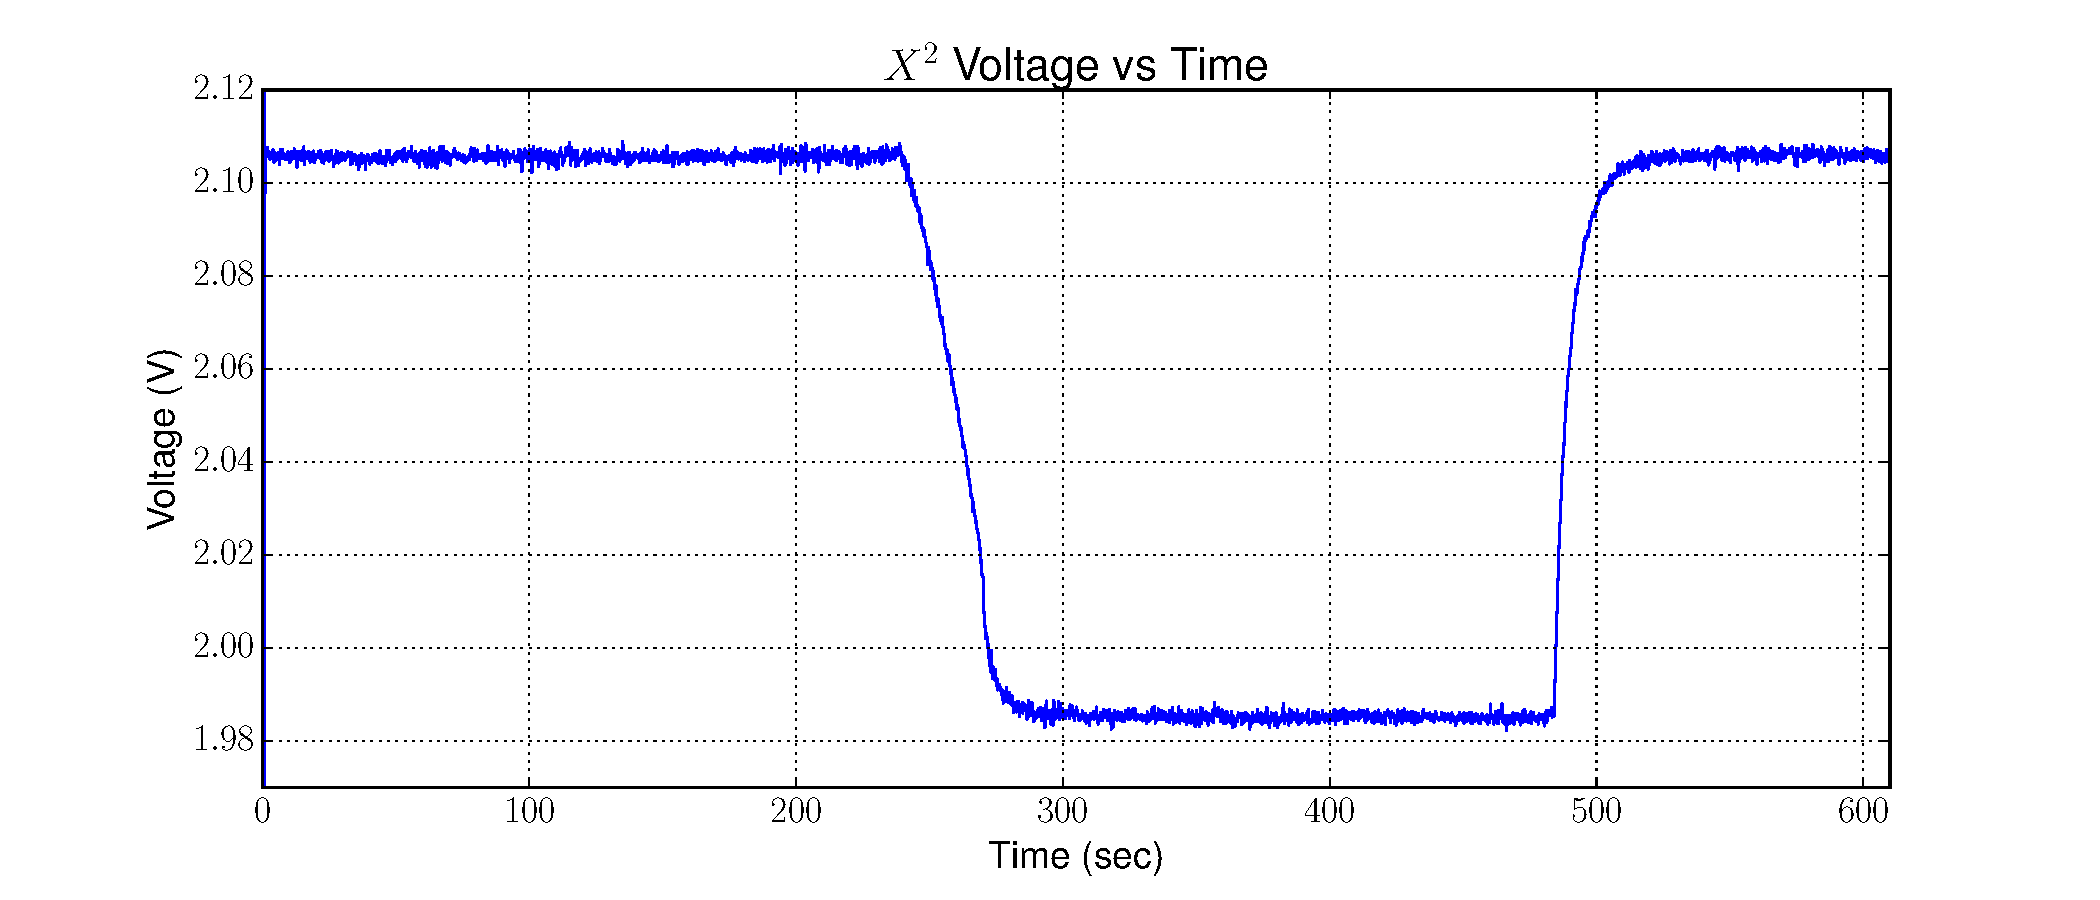
\includegraphics[width=\textwidth]{Experiments/Exp1/x2_filter.pdf}
\isucaption{Filtered data from the square-law detector used in Experiment I}
\label{X2_filter}
\end{figure}

Figure \ref{X2_filter} shows our data after being filtered by the low pass filter.  Using the same technique as earlier, we can now calibrate the raw voltages from the square-law detector to the noise temperature.  As with thte data collected from the SDR-based radiometer, the data from the square-law detector is calibrated to the physical temperature that our matched load is placed in.  Figure \ref{X2_Calibrated} shows the calibrated data from the square-law detector.  This now allows us to directly compare the square-law detector to the software defined radio data since we have a common reference point.

\begin{figure}[h!tb] \centering
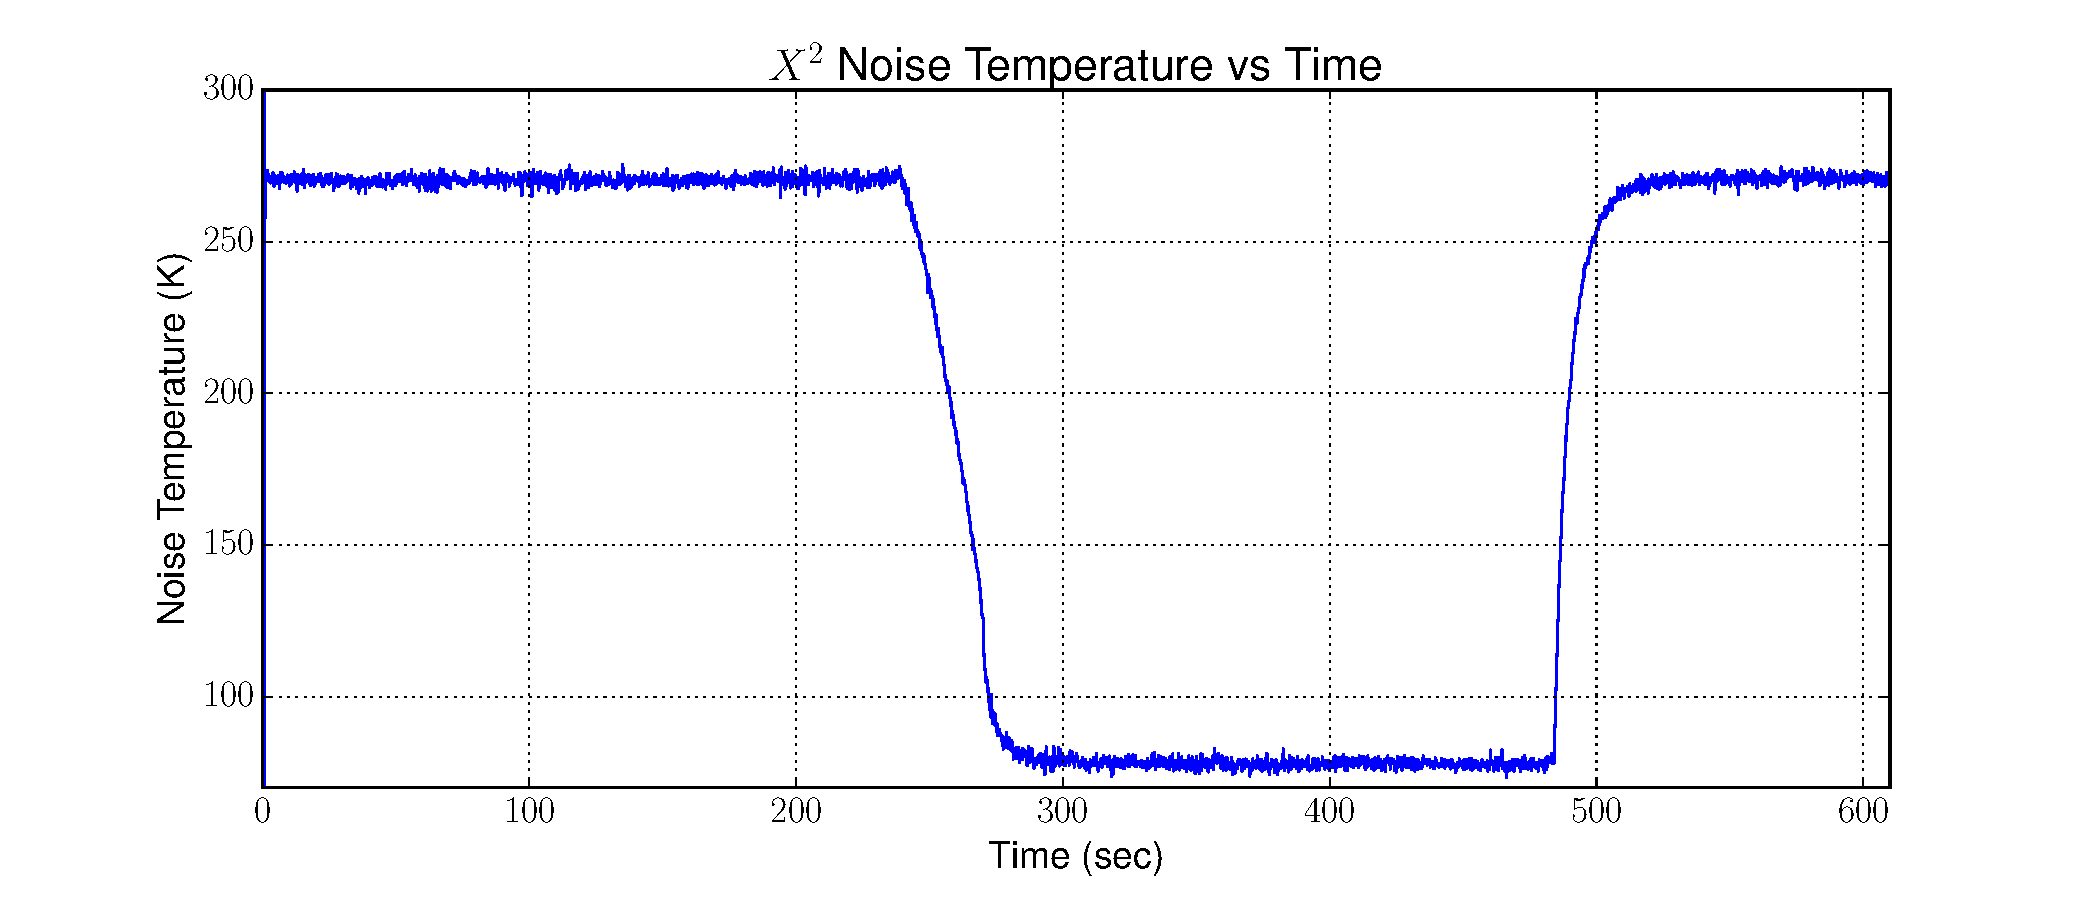
\includegraphics[width=\textwidth]{Experiments/Exp1/x2_calibrated.pdf}
\isucaption{Calibrated data from the square-law detector used in Experiment I}
\label{X2_Calibrated}
\end{figure}

\emph{SDR-based radiometer vs square-law detector.}  We now compare the Software Defined Radio Based Radiometer with the square-law to make sure they match.  Because both the SDR-Based Radiometer and the square-law are now calibrated to a noise temperature, we can graph both sets of data and compare them to each other.

\begin{figure}[h!tb] \centering

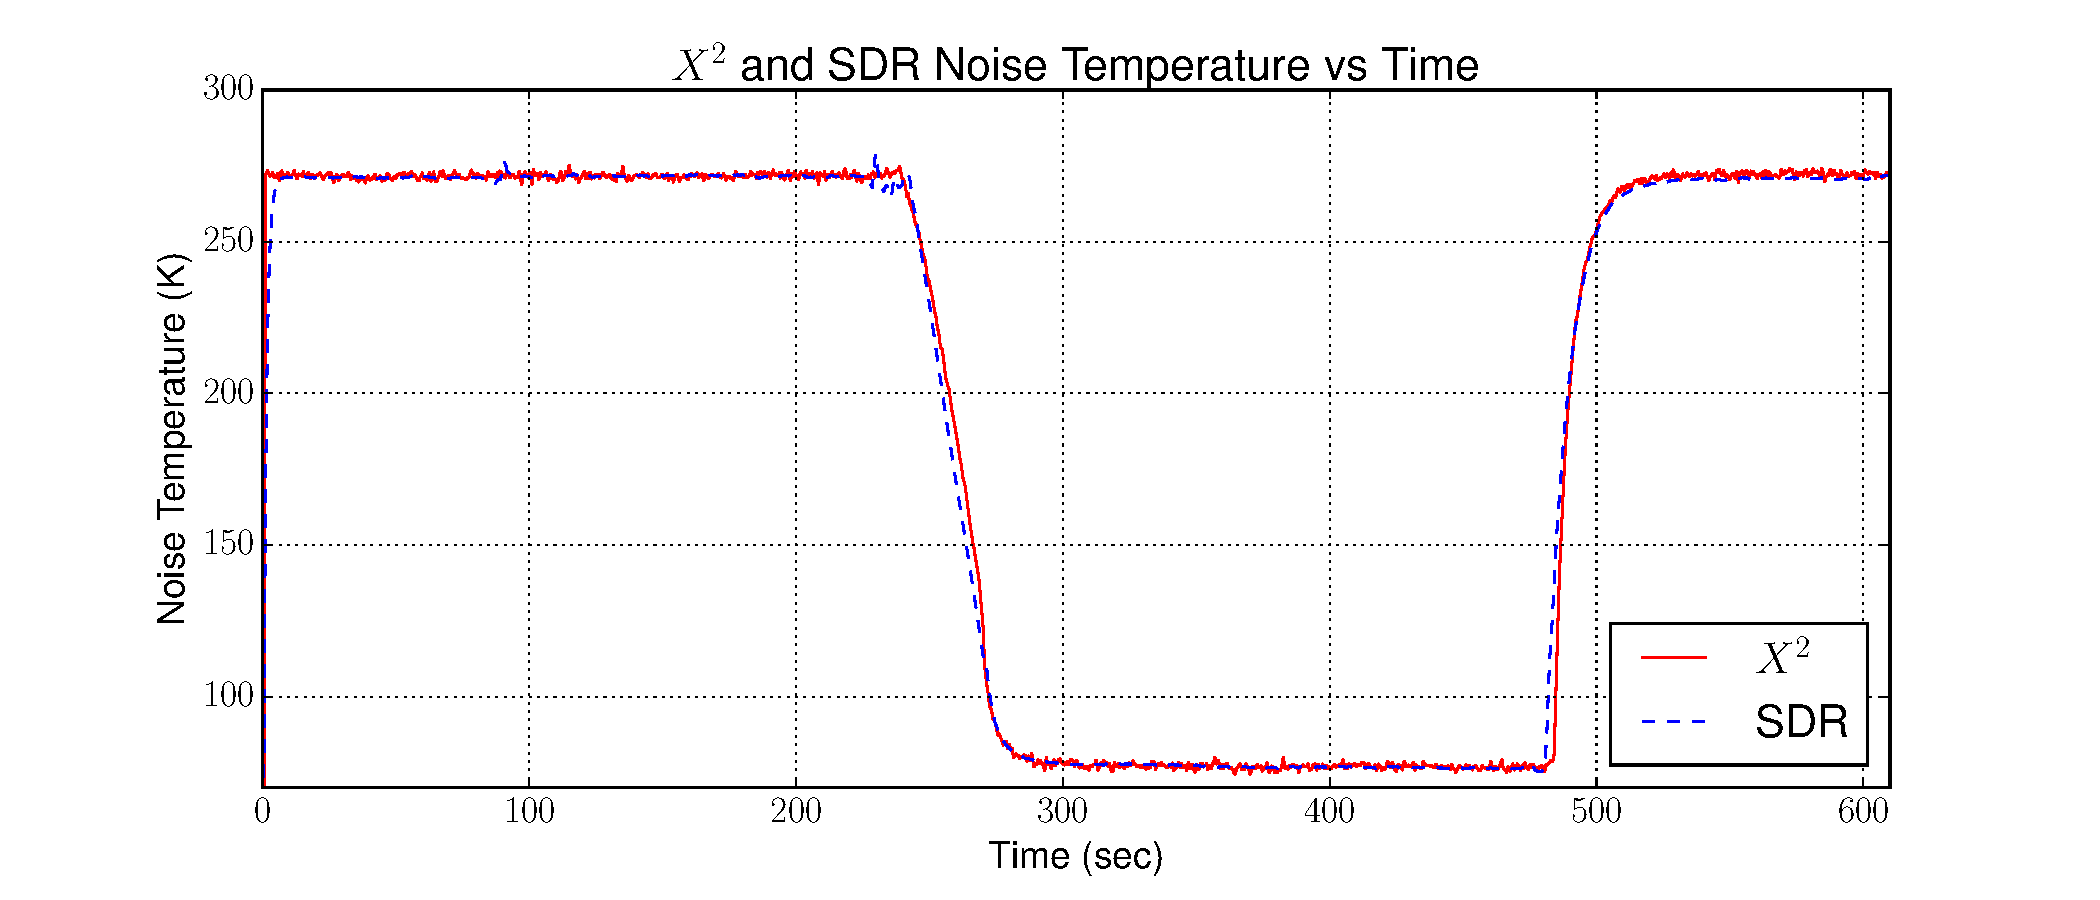
\includegraphics[width=\textwidth]{Experiments/Exp1/x2_SDR_Calibrated.pdf}
\isucaption{Figure showing both the SDR and square-law noise temperature data in Experiment I}
\label{X2_SDR_Both}
\end{figure}

We can see in Figure \ref{X2_SDR_Both} that both the software defined radio and the square-law detector match up very nicely.  This shows that both the square-law detector and the software defined radio agree when properly calibrated.  This verifies that the software defined radio can indeed operate as a total power radiometer and the data we obtain from this setup agrees with an analog and more traditional radiometer.

\section{Experiment II - Evaluation of sensitivity and stability} \label{Exp2_results}

\subsection{Data Collected}
This experiment examines the sensitivity and stability of a SDR-based radiometer.  The data used for the sensitivity is the same data collected in experiment one in section \ref{Exp1_data}.  The data collected for the stability is the total power data collected from the SDR-based radiometer over a period of 15 minutes.  For the sensitivity data, the data is calibrated using Table \ref{exp1_datapoints}.  For the stability data it is calibrated using Table \ref{exp2_datapoints}.

\begin{table}[h!tb] \centering
\isucaption{Total Power calibration data points for the stability experiment}
\label{exp2_datapoints}
% Use: \begin{tabular{|lc|} to put table in a box
\begin{tabular}{lc} \hline
\textbf{rQ Value} & \textbf{Temperature (K)} \\ \hline
.1132 & 77 \\
.1770 & 271.65 \\ \hline
\end{tabular}
\end{table}
 
\subsection{Data Analysis}\label{Exp2_analysis}

\emph{Sensitivity.}  Sensitivity for a radiometer is the $NE\Delta T$ that was covered in chapter \ref{ch:background} and is found in Equation \ref{NEAT_EQ}.  The sensitivity can also be measured as the standard deviation of the data that we collect from the software defined radiometer.  

\begin{table}[h!tb] \centering
\isucaption{Experimental parameters for experiment one.}
\label{exp2_param}
% Use: \begin{tabular{|lcc|} to put table in a box
\begin{tabular}{ccc} \hline
\textbf{Bandwidth ($\beta$)} & \textbf{Integration Time ($\tau$)} & \textbf{$T_{A}+T_{N}$}\\ \hline
10 MHz & 2 sec & 427 K \\ \hline
\end{tabular}
\end{table}

Python is used to calculate the $NE\Delta T$ using the data from Table \ref{exp2_param}.  The python code listed below is used to calculate the theoretical $NE\Delta T$.

\begin{lstlisting}[frame=single,keywordstyle=\color{blue}]
tau = 2 # Integration Time
BSDR = 10e6 # Bandwidth
TN = 385 # System noise temperature
TA = 77 # Antenna noise temperature
NEAT_SDR = (TA+TN)/sqrt(BSDR*tau)
\end{lstlisting}

This gives us 0.1 Kelvin for the expected $NE\Delta T$.  Since the sensitivity is related to the standard deviation of the graph, we can use Python to give us the standard deviation of the data graphed in Figure \ref{Sensitivity_graph}.  Figure \ref{Sensitivity_graph} uses the data graphed in \ref{SDR_Calibrated} but zoomed in from 350 to 450 seconds. 

\begin{figure}[h!tb] \centering
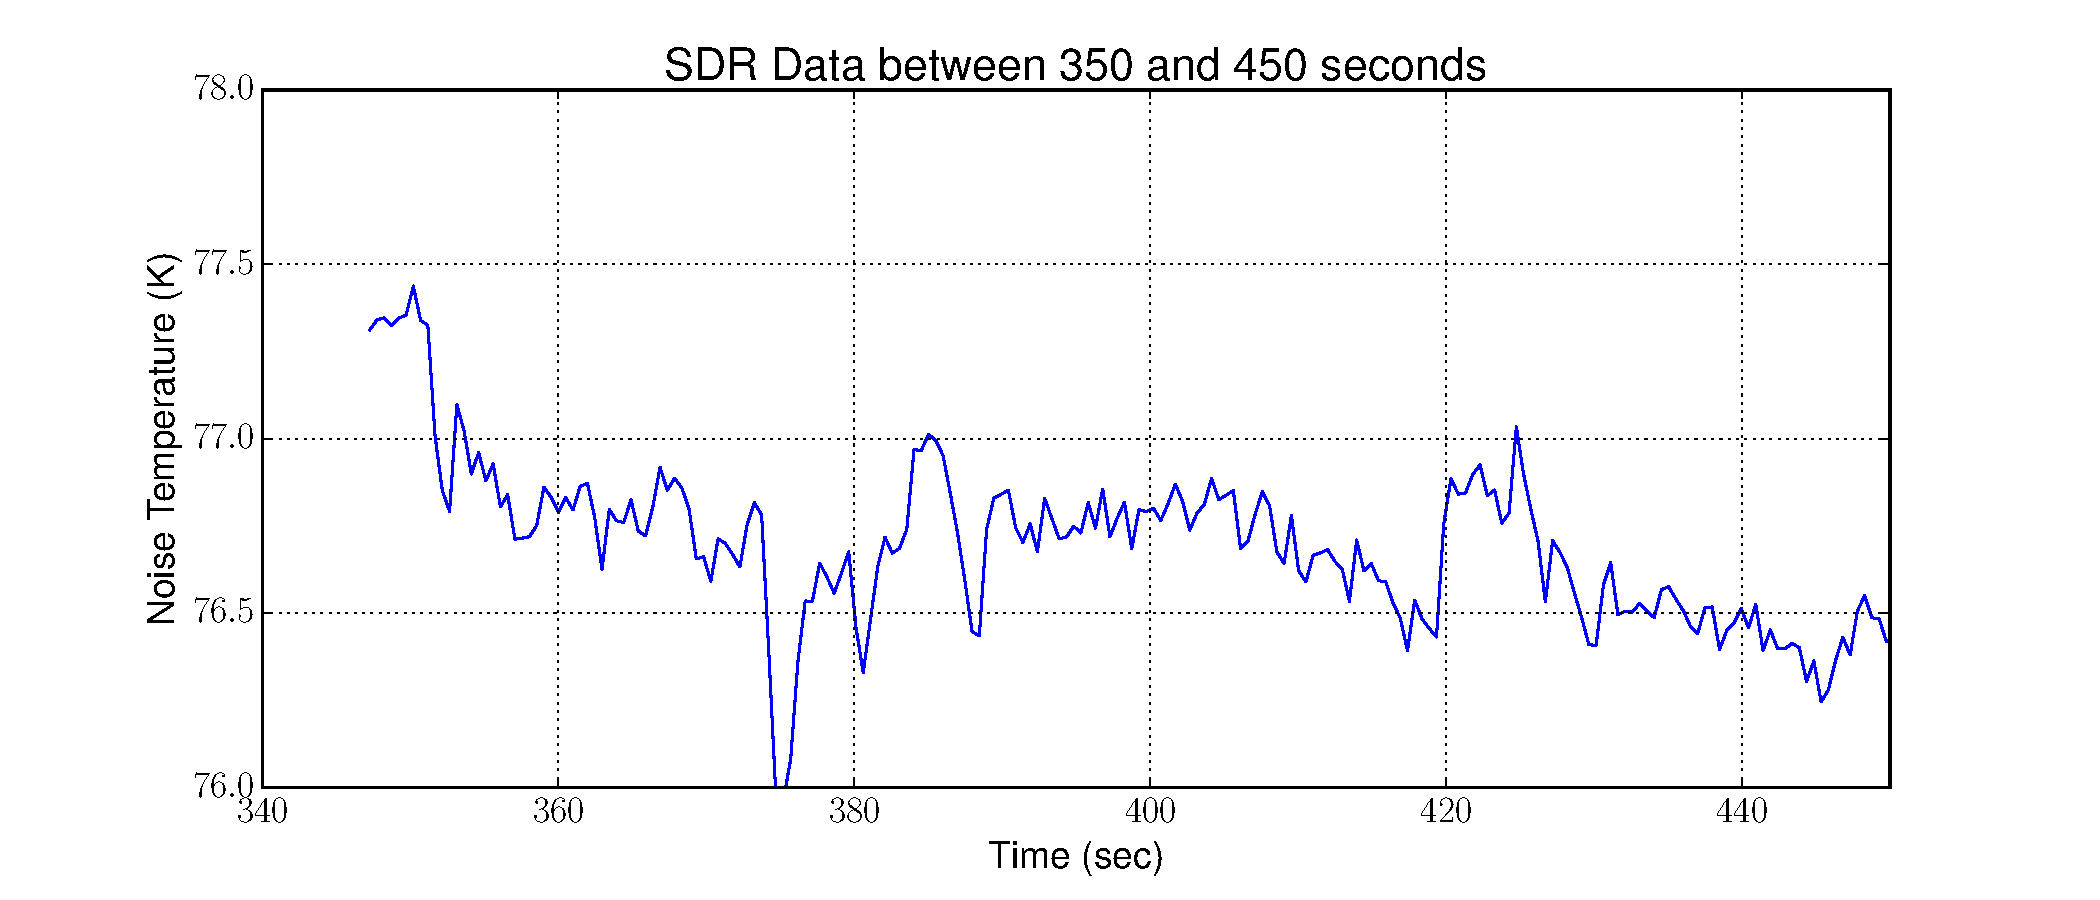
\includegraphics[width=\textwidth]{Experiments/Exp1/SDR_Zoom.pdf}
\isucaption{Graph of the calibrated total power from Experiment I while the matched load is submerged in LN2 between 350 and 450 seconds.}
\label{Sensitivity_graph}
\end{figure}

Python is used to determine the standard deviation of this range of data.  The code used is shown below and gives a result of .23 Kelvin.  We can now plot both the expected sensitivity and the actual sensitivity which is shown in Figure \ref{sensitivity_exp_real}.

\begin{lstlisting}[frame=single,keywordstyle=\color{blue}]
stdsdr = numpy.std(g)
print stdsdr
\end{lstlisting}

\begin{figure}[h!tb] \centering
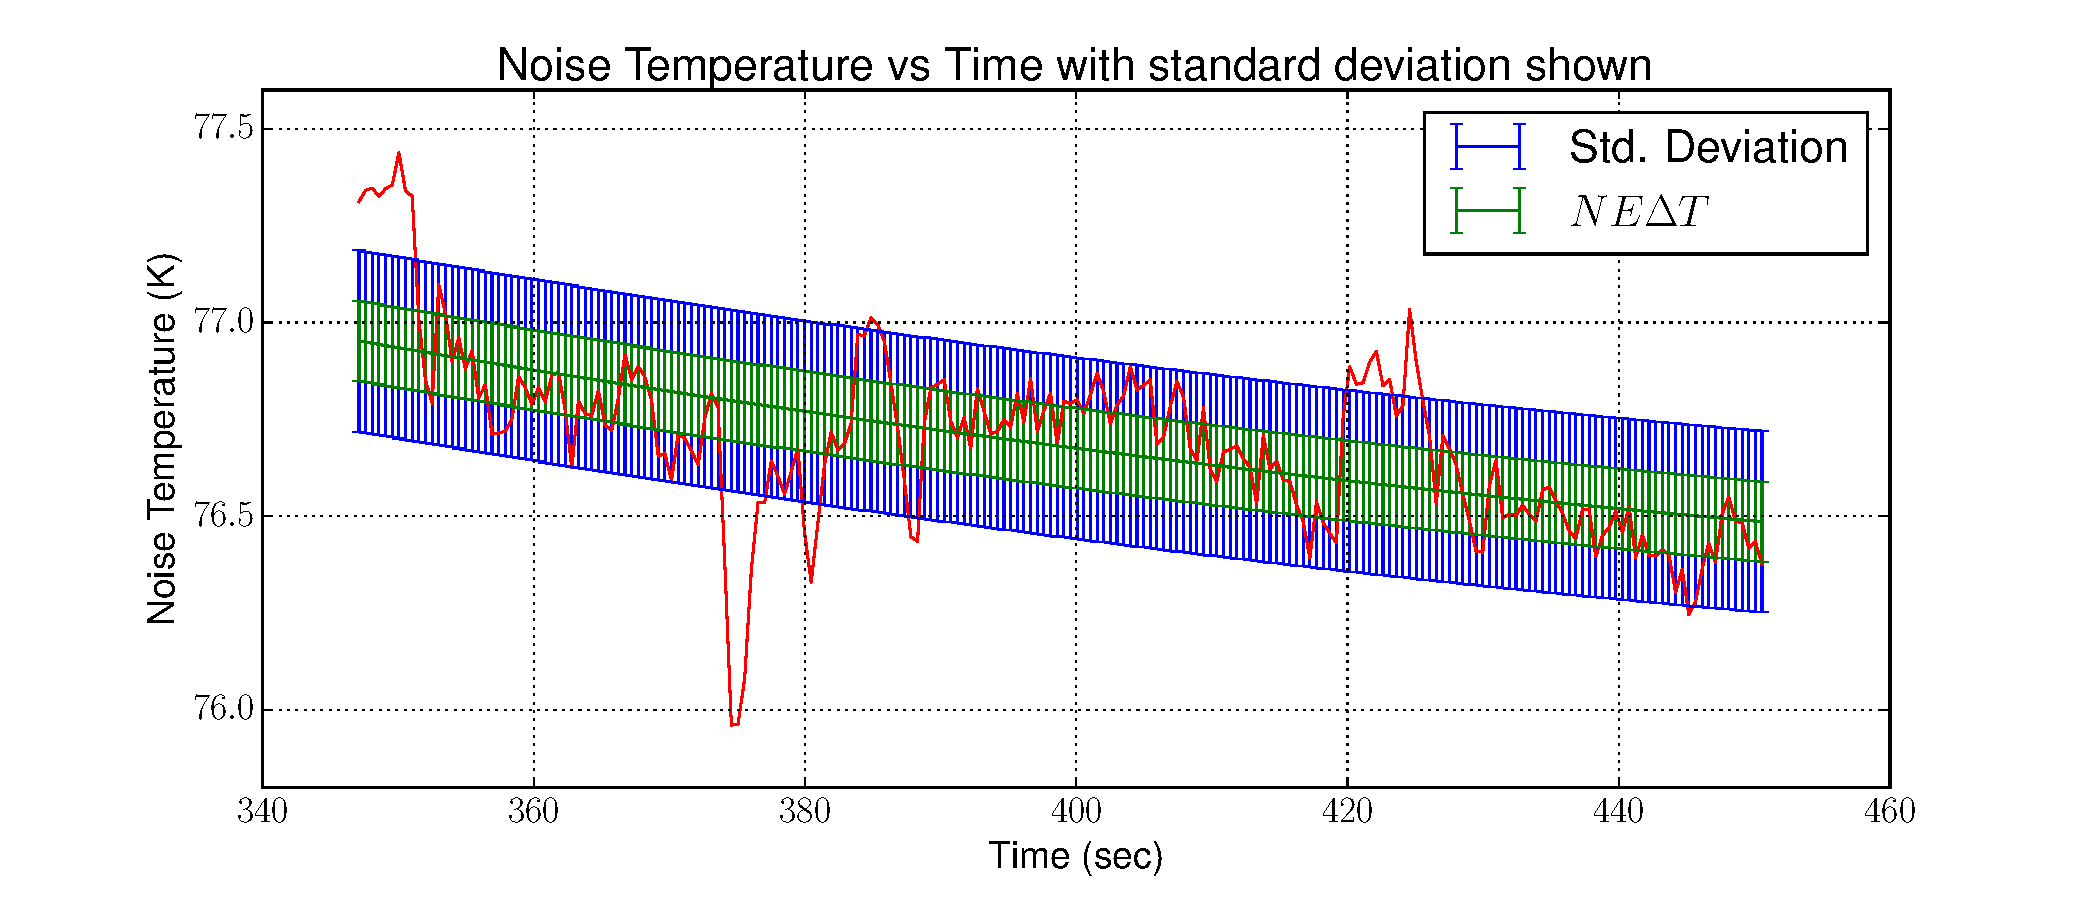
\includegraphics[width=\textwidth]{Experiments/Exp1/std_dev_errbar.pdf}
\isucaption{Graph of the calibrated total power with expected and actual sensitivity.}
\label{sensitivity_exp_real}
\end{figure}

While .23 Kelvin is higher than the calculated sensitivity, it is still quite acceptable.  As discussed in chapter \ref{ch:implementation} and shown in Table \ref{rad_performance}, our target $NE\Delta T$ is one Kelvin or less.  Therefore our actual performance of .23 Kelvin still meets our radiometer requirement.

\emph{Stability.}  To verify stability of the radiometer, we look to see how much change the radiometer records over a relatively long period of time.  To test this, a matched load was submerged in a liquid nitrogen bath for an extended period of time, in this case for fifteen minutes.  The readings were then examined to study the trend of the data.  The data is graphed in Figure \ref{Stability}.

\begin{figure}[h!tb] \centering
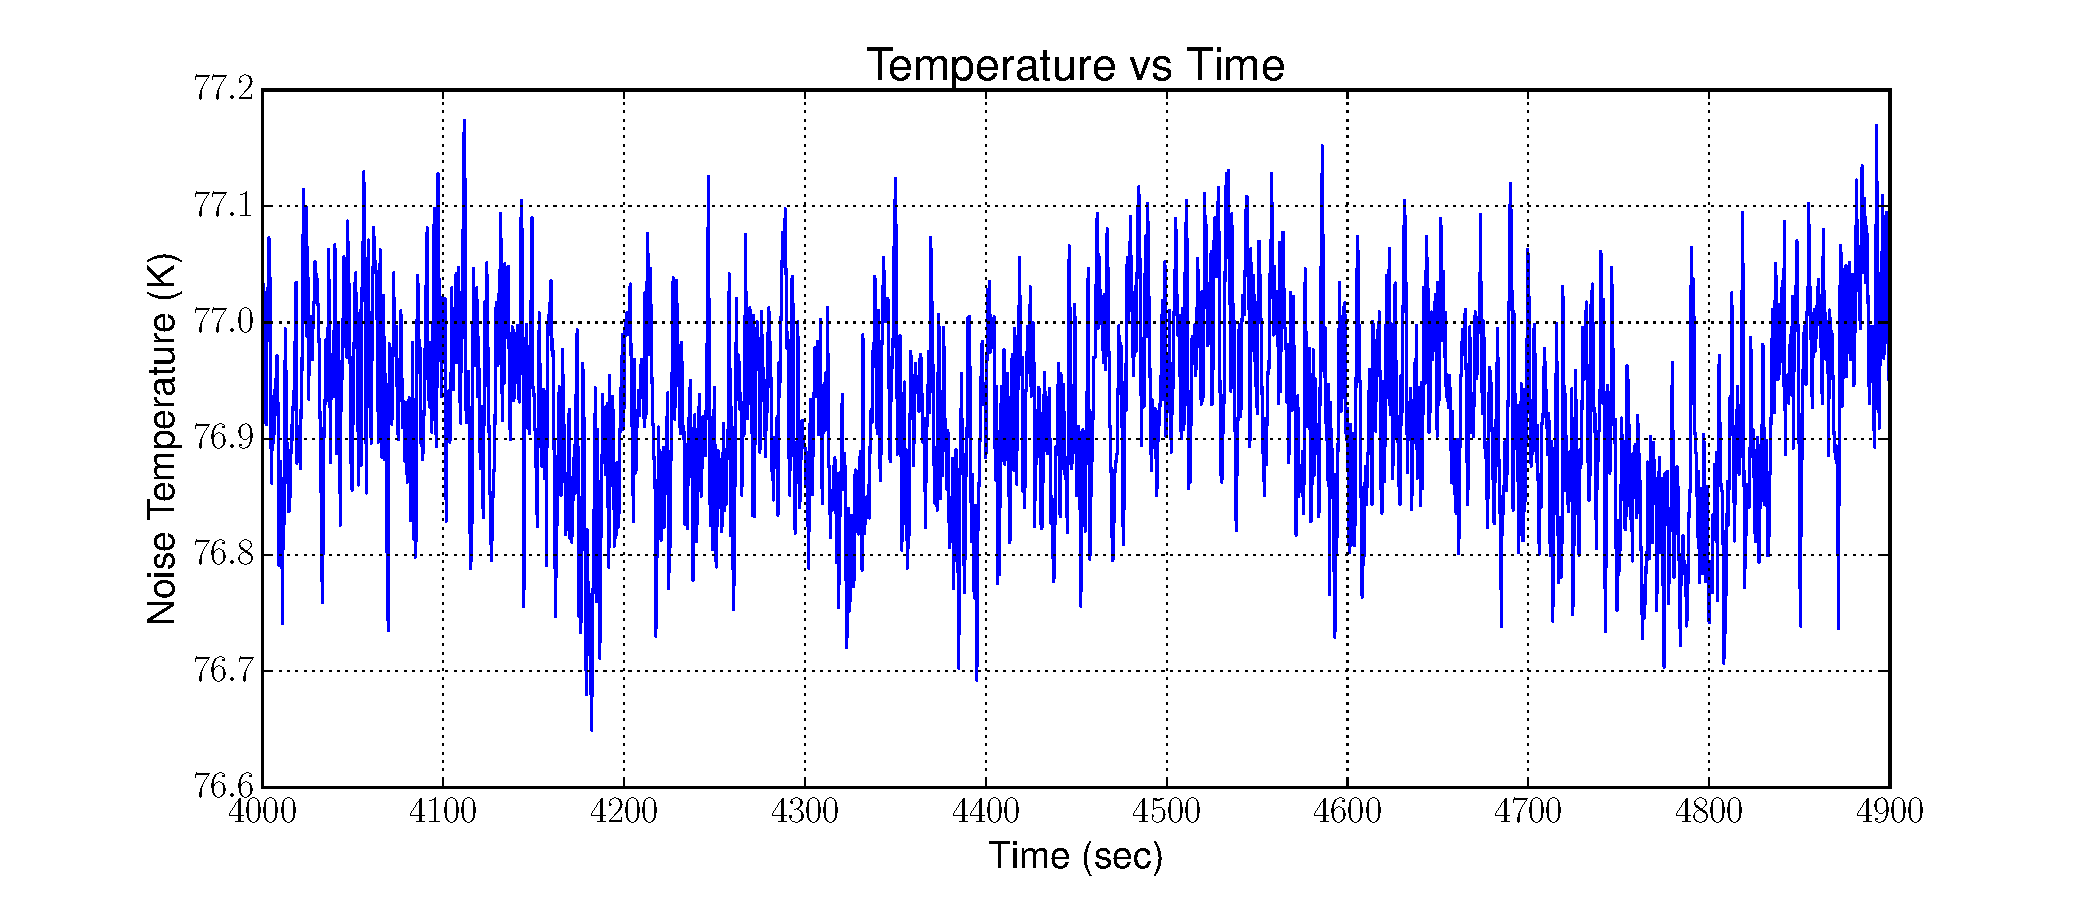
\includegraphics[width=\textwidth]{Experiments/Exp2/sdr_calibrated_zoom.pdf}
\isucaption{Graph of the calibrated total power over a period of fifteen minutes.}
\label{Stability}
\end{figure}

We can use Python to calculate a second order polynomial to create a line to fit the data in Figure \ref{Stability}.  An ideal line would be flat to show no overall change with the data.  In Figure \ref{Stability_calib} we can see that the line and the data does not change more than 0.05 Kelvin over this fifteen minute period.

\begin{figure}[h!tb] \centering
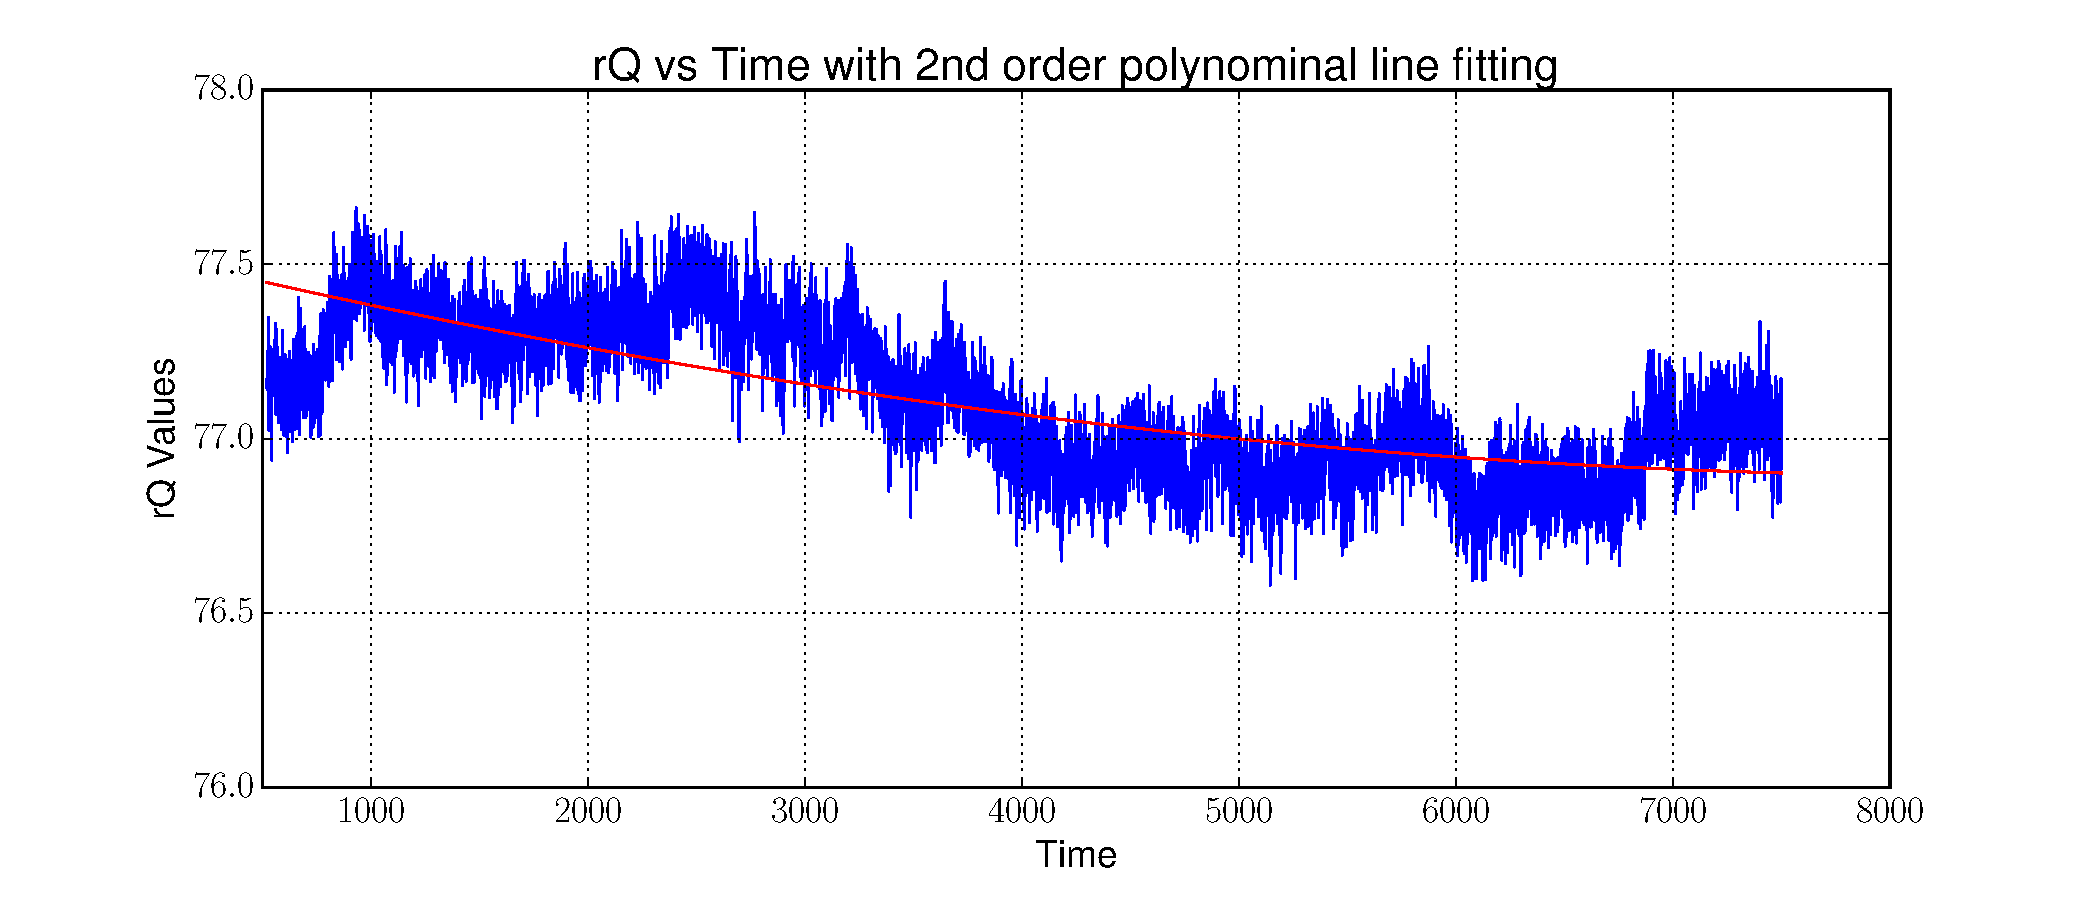
\includegraphics[width=\textwidth]{Experiments/Exp2/calib_line_fitting.pdf}
\isucaption{Graph of the calibrated total power over a period of 15 minutes with a best fitted line.}
\label{Stability_calib}
\end{figure}

\section{Experiment III - Interfering Signal Mitigation} \label{Exp3_results}

The addition of a unwanted interfering signal has an adverse effect on how a radiometer operates[\cite{Ellingson}].  This is a growing problem for all radiometers, but is a greater issue for radiometers used in orbiting spacecrafts to observe the Earth as they see large areas that could contain interfering signal sources [\cite{DeRooRFI}].  Even though the band we are working in (i.e. 1.4 GHz) is an internationally protected frequency, there have been both intentional and unintentional signal sources in this band detected by current space borne radiometers that have caused interference [\cite{Forte}].

\subsection{Data Collected}

The data collected for Experiment III is the total power values from the SDR-based radiometer and the voltage data from the square-law detector.  These values are calibrated using the data points provided in Table \ref{exp3_datapoints}.  These values differ from the previous tables because the filter is turned on.  This changes the performance of the SDR-based radiometer and results in different rQ values.  The voltages are higher due to the presence of the offending signal.

\begin{table}[h!tb] \centering
\isucaption{Total Power calibration data points}
\label{exp3_datapoints}
% Use: \begin{tabular{|lcc|} to put table in a box
\begin{tabular}{lcc} \hline
\textbf{rQ Value} & \textbf{$X^2$ Voltage (V)} & \textbf{Temperature (K)} \\ \hline
.0361 & 2.1234 & 77 \\
.0623 & 2.1872 & 271.65 \\ \hline
\end{tabular}
\end{table}

\subsection{Data Analysis}

We begin by looking at what happens to our total power readings when no RFI mitigation is used.  As we stated in Section \ref{exp3_setup}, the frequency of the offending signal will not change, but the amplitude will.  This results in clear indications of the total power changing as the amplitude of the offending signal changes.  

\begin{figure}[h!tb] \centering
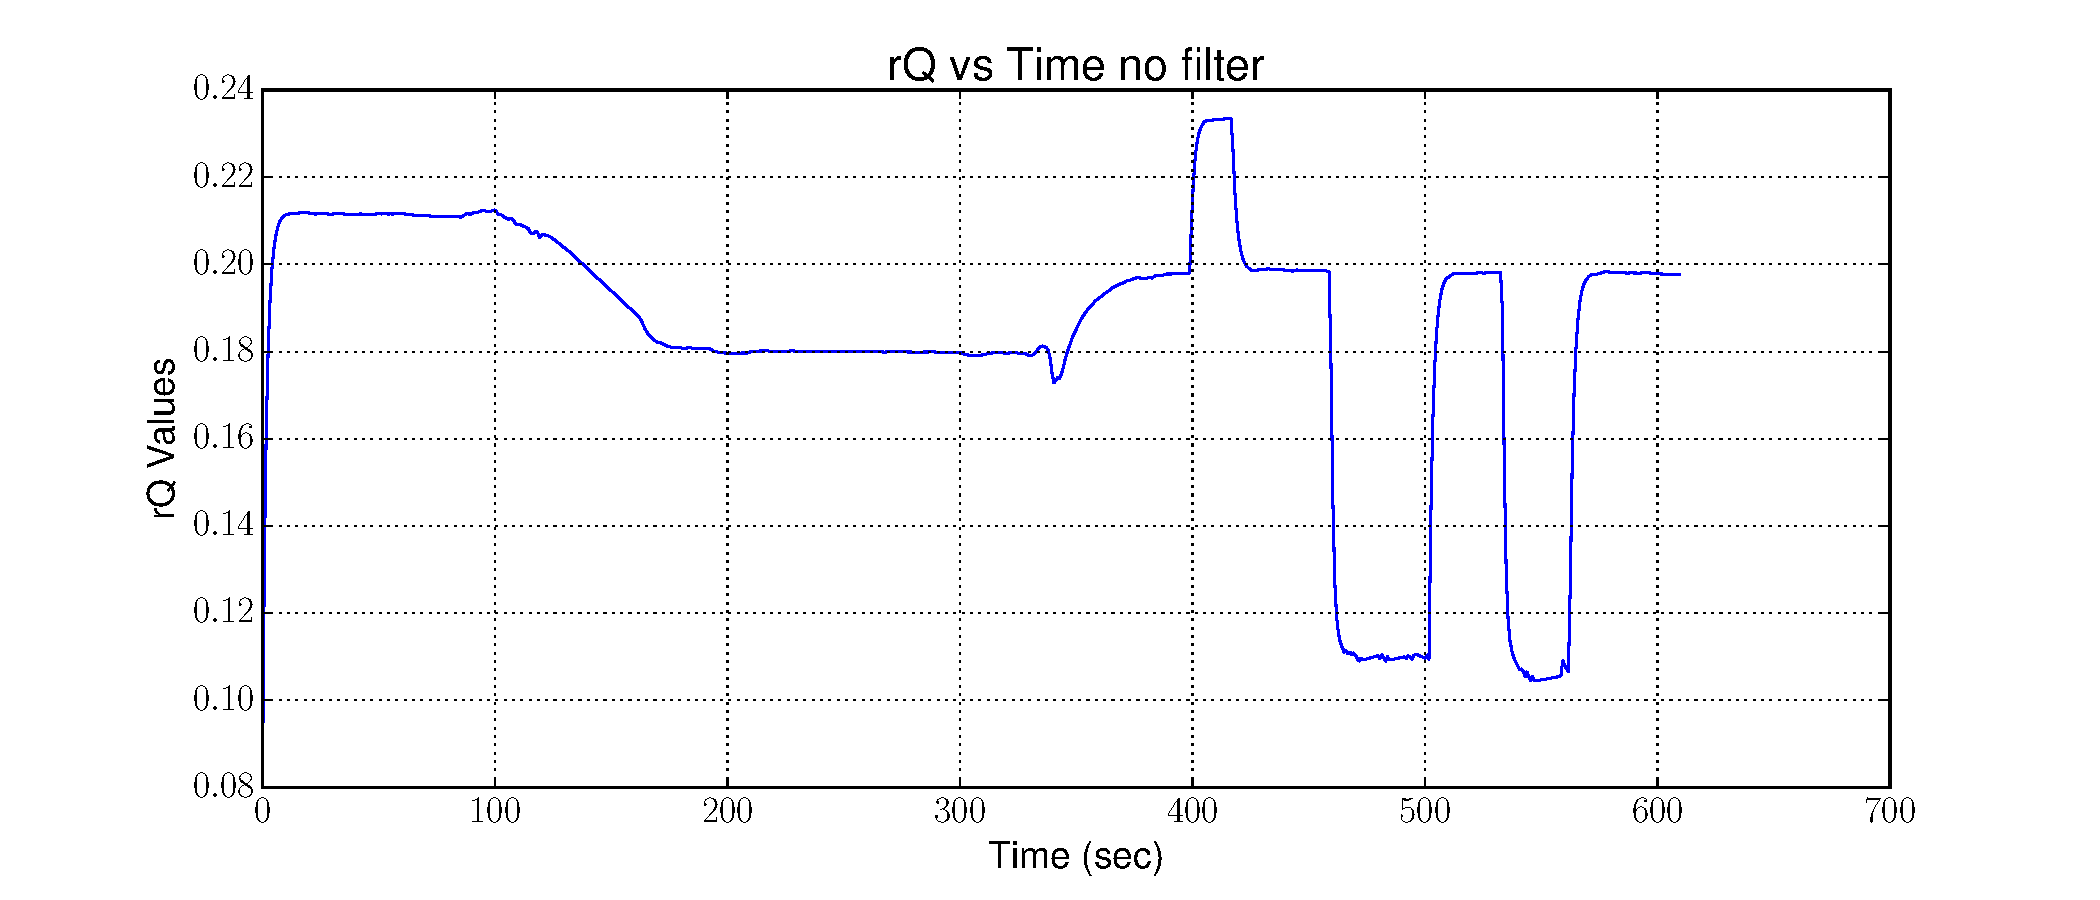
\includegraphics[width=\textwidth]{Experiments/Exp4/sdr_raw_unfiltered.pdf}
\isucaption{Graph showing the unfiltered total power measurements of the software defined radio}
\label{sdr_unfilt_raw}
\end{figure}

It can be seen that there are pulses that occur in Figure \ref{sdr_unfilt_raw} that correspond to changes in the amplitude of the offending signal that affect our total power readings.  These same pulses can be seen in the square-law detector data shown in Figure \ref{x2_unfilt_signal}.

\begin{figure}[h!tb] \centering
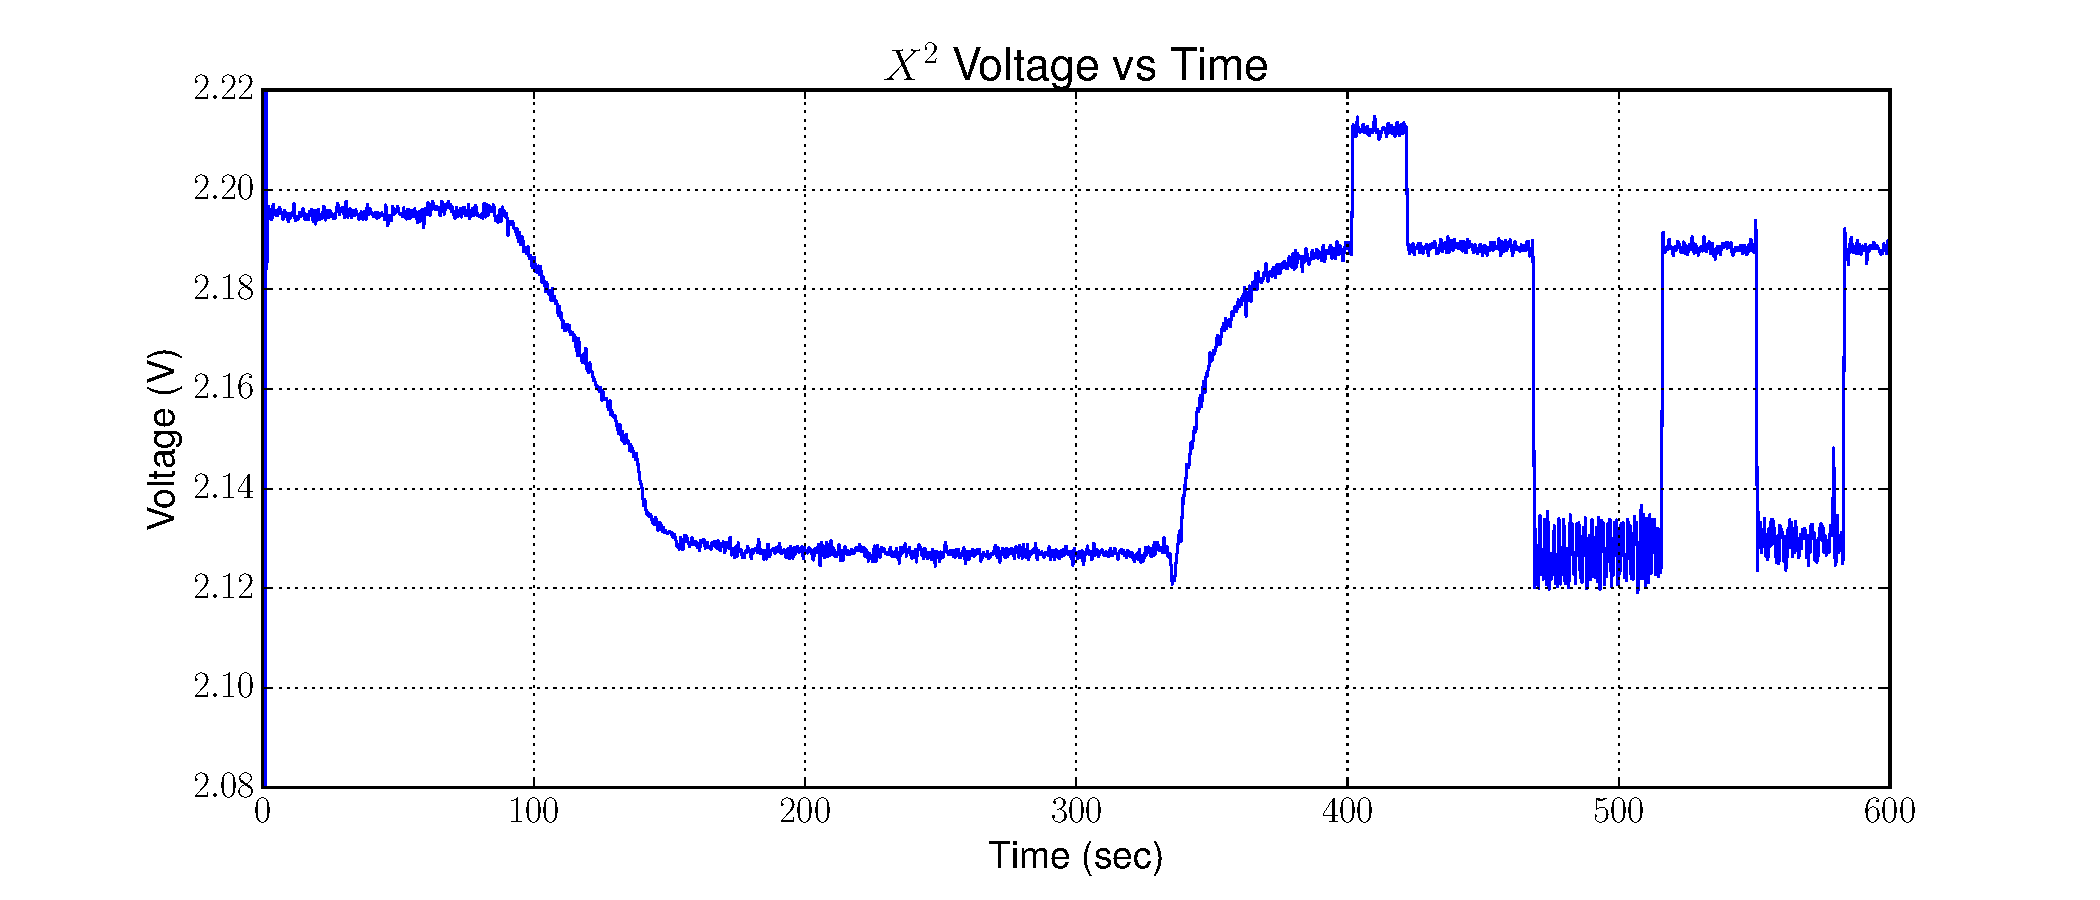
\includegraphics[width=\textwidth]{Experiments/Exp4/x2_voltage.pdf}
\isucaption{Graph showing the raw total power read from the square-law detector with an interfering signal.}
\label{x2_unfilt_signal}
\end{figure}

We can see in both the software defined radio and the square-law detector that there is an interfering signal.  If we now look at the spectrum view of the software defined radio, shown in \ref{spectrum_interfering}, we can see the signal in question occurs  at 1.405 GHz.  The square-law detector has no frequency information, so our only method to detect an interfering signal is by looking at the total power readings.  In Figure \ref{x2_unfilt_signal} we can see the spikes in the square-law data, however, we do not know where in the spectrum the offending signal is located.

\begin{figure}[h!tb] \centering
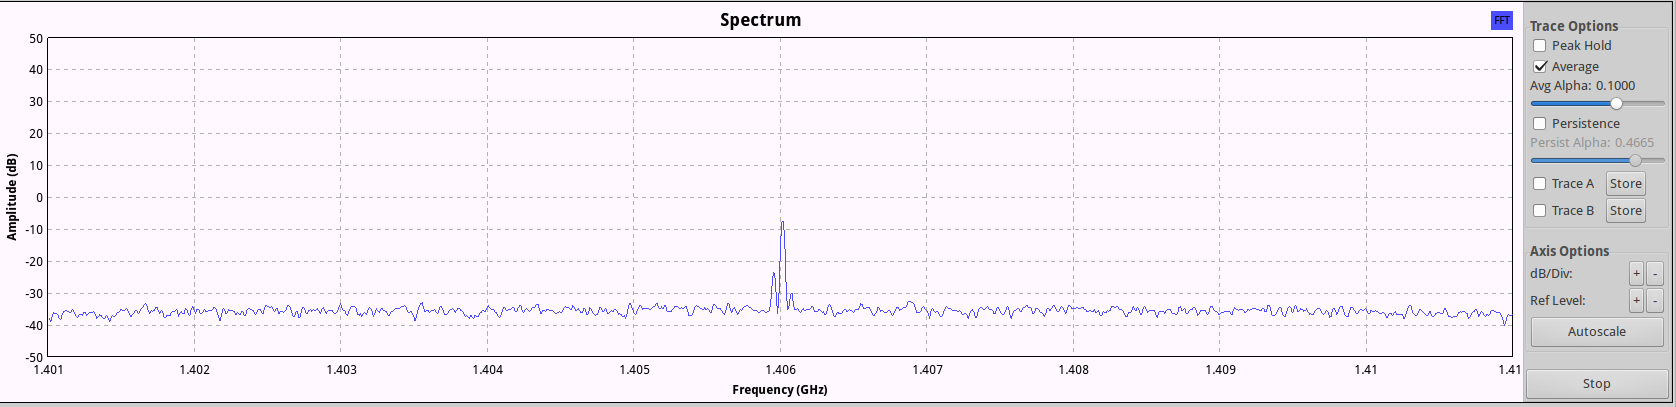
\includegraphics[width=\textwidth]{Images/interfering_signal_filter.png}
\isucaption{Image showing the spectrum view of the SDR-based radiometer with no RFI mitigation.}
\label{spectrum_interfering}
\end{figure}

Since we know where the offending signal is located for the SDR-based radiometer, we can design a filter to remove this signal.  In GNURadio, we can specify both the frequency and the bandwidth that we desire for this band-reject filter.  Ideally we want to keep the bandwidth of the filter as tight as possible to the offending signal, while making sure our filter is effective in removing the signal.  Figure \ref{spectrum_filter} shows the spectrum display of the software defined radio while filtering the offending signal.

\begin{figure}[h!tb] \centering
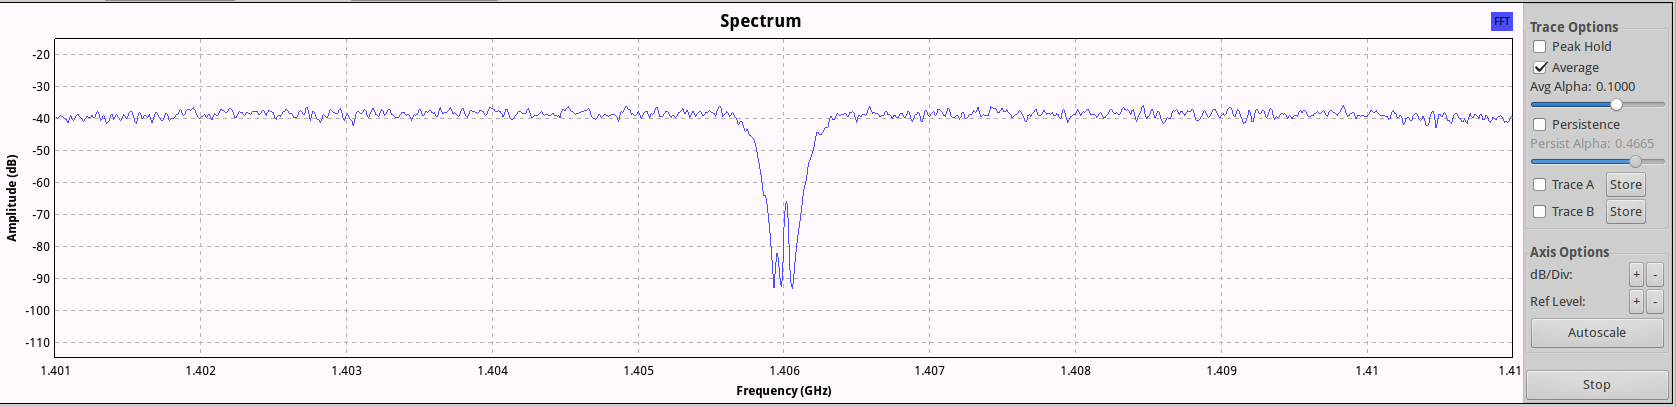
\includegraphics[width=\textwidth]{Images/interfering_signal.png}
\isucaption{Image showing the spectrum view from the SDR-based radiometer filtering the offending signal}
\label{spectrum_filter}
\end{figure}

Since we have now removed the offending signal, we want to re-run our experiment and once again compare the difference between the software defined radio and the square law detector. We can begin by looking at the software defined radio total power readings.  Figure \ref{sdr_calib_filter} shows a calibrated graph of the noise temperature seen by the software defined radio.  This graph is similar to graphs we expect from a total power radiometer.  However, we want to compare this to our square-law detector as well.  

\begin{figure}[h!tb] \centering
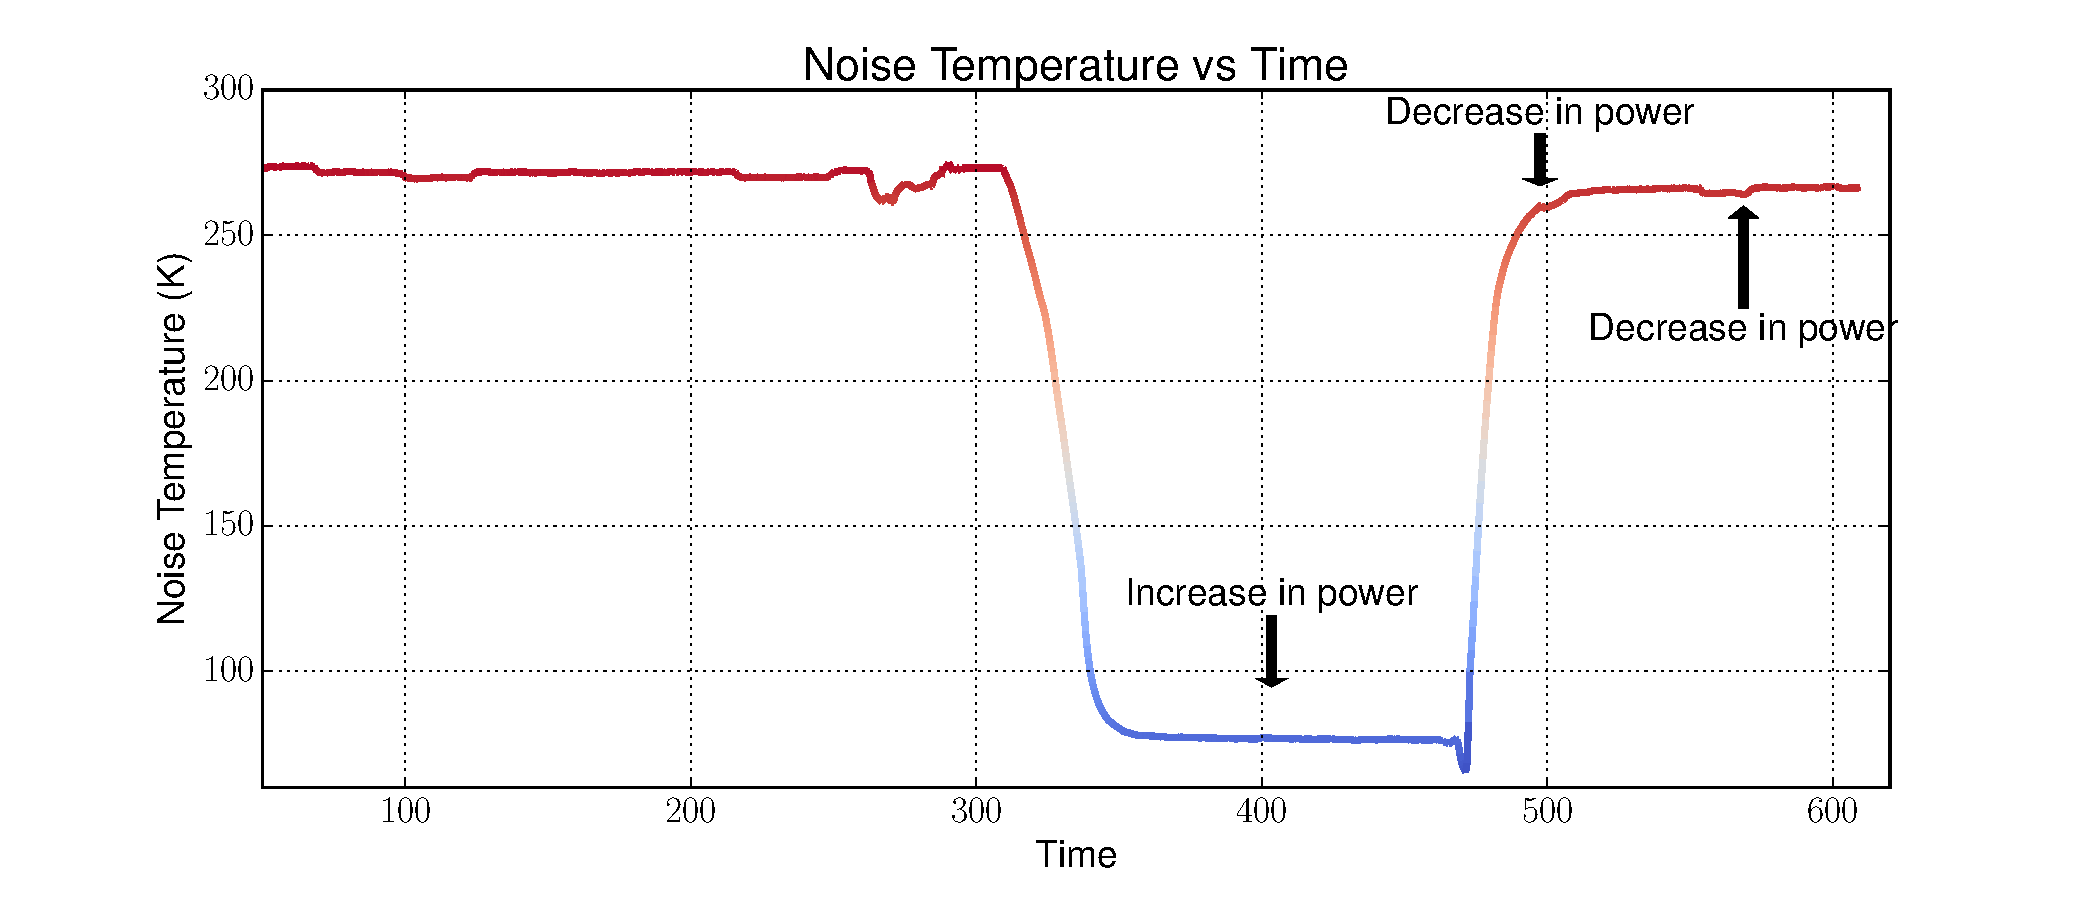
\includegraphics[width=\textwidth]{Experiments/Exp4/calib_filtered.pdf}
\isucaption{Graph showing the calibrated total power readings with the filter removing the offending signal}
\label{sdr_calib_filter}
\end{figure}

Figure \ref{filter_on} shows both the software defined radio and the square-law detector calibrated total power readings.  In this graph you can see that the software defined radio is able to make normal readings where the square-law detector still shows changes in amplitude corresponding to offending signal pulses, which would make both calibration and obtaining useful data difficult.

\begin{figure}[h!tb] \centering
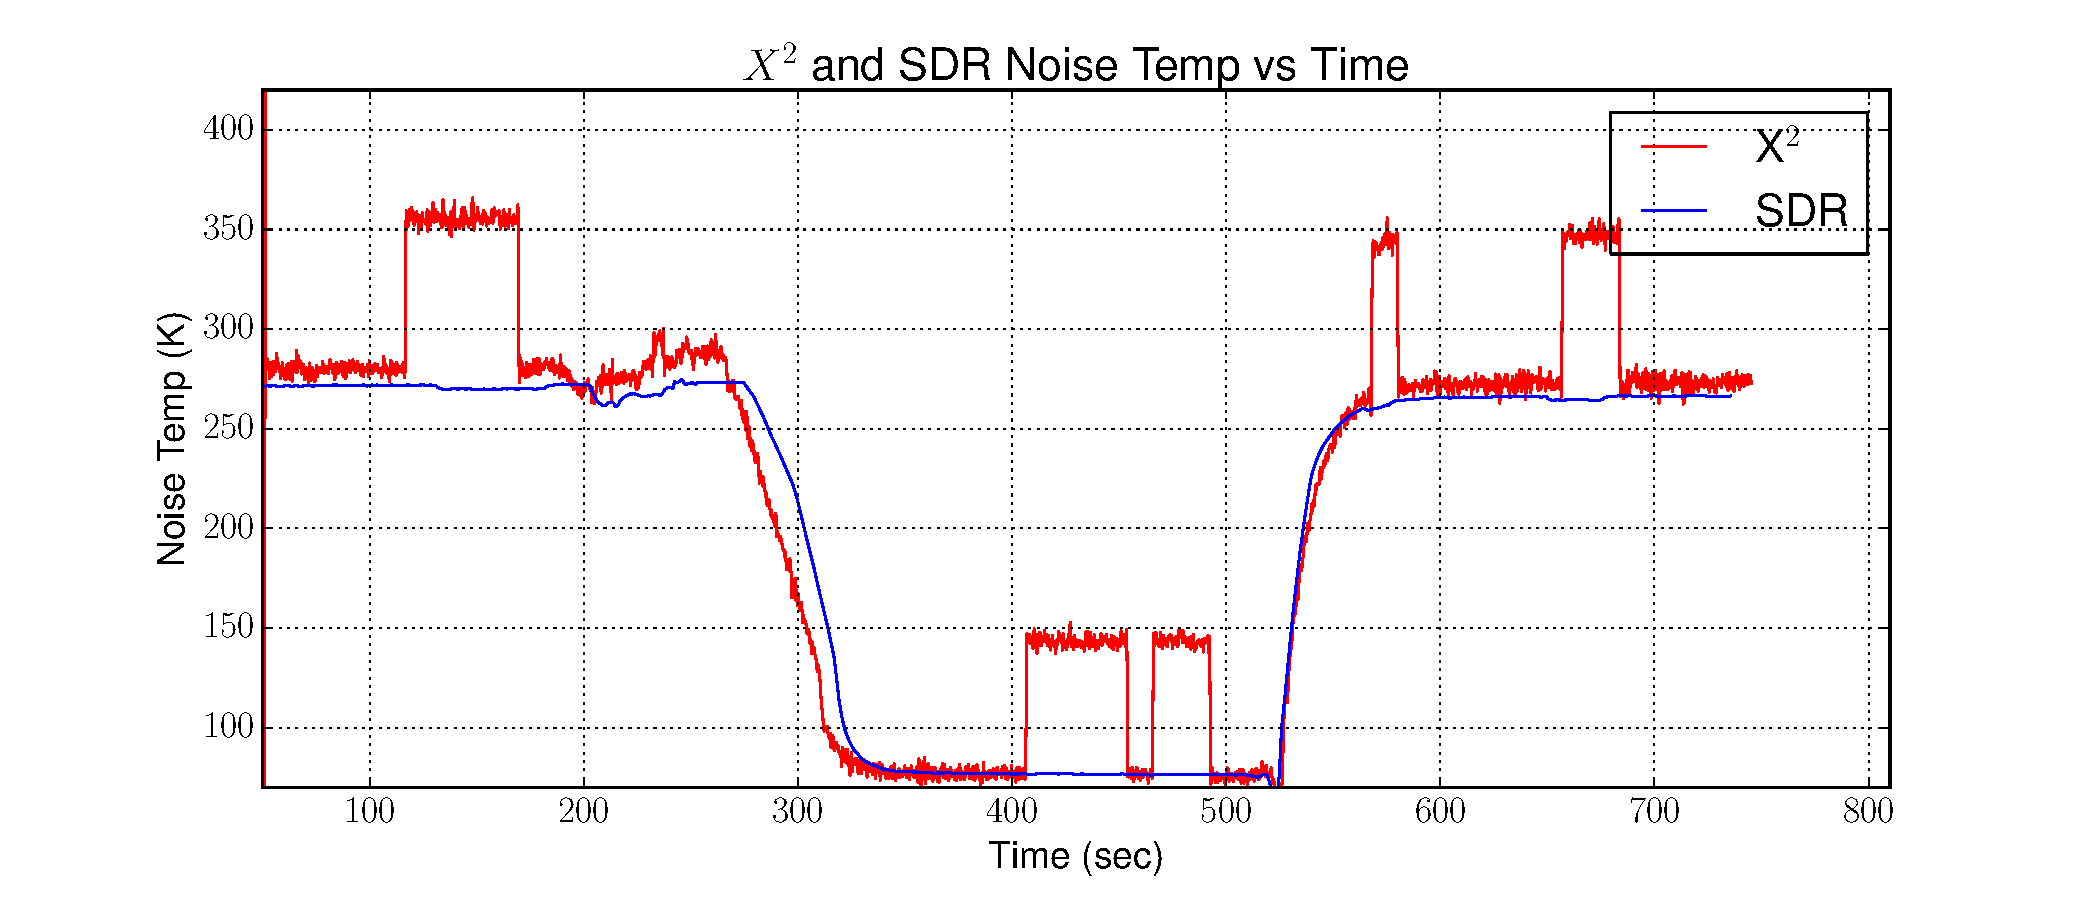
\includegraphics[width=\textwidth]{Experiments/Exp4/calib_filtered_both.pdf}
\isucaption{Image of the offending signal being filtered out by the SDR.  It can be seen that the signal is no longer visible.}
\label{filter_on}
\end{figure}

\emph{Filter delay.}  It should be noted that when doing data analysis, that there will be some delay due to two factors.  First, there is a delay in the software defined radiometer due to the integrator that is used.  This creates a time delay as the integrator accumulates information and then settles.  We use fairly large integration times, usually in seconds so this can add a significant delay.  Second we do have a smaller delay in the decimation and low pass filter also used in the software defined radiometer.  These are Finite Impulse Response (FIR) filters and thus have a delay given in Equation \ref{FIR_delay}, where $N$ is the number of taps generated and $F_{s}$ is our sampling frequency, in our case 10 MHz.

\begin{equation}\label{FIR_delay}
\frac{(N - 1)}{(2*F_{s})}
\end{equation}

The taps value is generated by Python using the filter design program.  For this experiment, the number of taps generated was 18,181.  Taking this and our sampling rate into account, our FIR filter only delays the signal by 9 milliseconds.  

A final note on aligning the square-law detector and the software defined radiometer data.  Both systems have a record function and must be started manually by the user.  They also run on separate computers.  Therefore, there is a human error that also gets introduced to the system as well.  This is usually no more than 1 or 2 seconds.  But in this experiment it was noted that there was a slightly longer delay between the two of about 4 seconds.  

\section{Experiment IV - Performance impact of interfering signal mitigation} \label{Exp4_results}
The goal of this experiment is to examine what affect adding a filter was on the performance of the radiometer.  While we have demonstrated we can filter an offending signal, this comes at a cost.  This experiment examines the impact filtering out bands has on the measurement of total power and radiometer sensitivity.

\subsection{Data Collected}
The data collected for this experiment is shown Table \ref{exp4_data_power} and Table \ref{exp4_datapoints}, and the remaining data is data generated from Equations \ref{NEAT_FILTER} and \ref{PWR_FILTER}.  This data will be examined next.

\begin{table}[h!tb] \centering
\isucaption{Measured sensitivity and Bandwidth of Filter}
\label{exp4_data_power}
% Use: \begin{tabular{|lc|} to put table in a box
\begin{tabular}{lc} \hline
\textbf{NEAT (K)} & \textbf{Bandwidth (MHz) } \\ \hline
.139 & .125 \\
.141 & .250 \\
.143 & .500 \\
.147 & 1 \\
.153 & 2 \\
.166 & 3 \\
.181 & 4 \\
.195 & 5 \\
.234 & 6 \\
.252 & 7 \\
.318 & 8 \\
.450 & 9 \\
1.45 & 10 \\ \hline
\end{tabular}
\end{table}

\begin{table}[h!tb] \centering
\isucaption{Measured Total Power and Bandwidth of Signal}
\label{exp4_datapoints}
% Use: \begin{tabular{|lc|} to put table in a box
\begin{tabular}{lc} \hline
\textbf{Total Power Value (rQ)} & \textbf{Bandwidth (MHz)} \\ \hline
.003 & .125 \\
.006 & .250 \\
.012 & .500 \\
.025 & 1 \\
.050 & 2 \\
.071 & 3 \\
.101 & 4 \\
.125 & 5 \\
.140 & 6 \\
.170 & 7 \\
.200 & 8 \\
.230 & 9 \\
.250 & 10 \\ \hline
\end{tabular}
\end{table}

\subsection{Data Analysis}

In Experiment IV, we examine the performance of a software defined radiometer when a filter is used.  Recalling the equation for $NE\Delta T$ from Equation \ref{NEAT_EQ}, our sensitivity is a function of the amount of noise from both the antenna ($T_{A}$) and the addition of system noise ($T_{N}$).  Sensitivity is also a function of the radiometer's bandwidth ($\beta$) and integration time ($\tau$).

Our integration time is controllable, and can be set using the GUI panel of the software defined radio.  In a typical radiometer, we often do not have any control of the bandwidth.  It is often set by the mechanical band-pass filters that are in place and the square-law detector circuit to measure the noise power.  In a SDR radio, we have more control over bandwidth as we can change our sampling rate which in turns controls our bandwidth.  There is a limit as larger sampling rates require higher performance ADCs and greater computing speed.

Recall from Experiment III, in section \ref{Exp3_results}, where we filtered out an offending signal.  While we were able to filter out the offending signal and resume total power measurements, it comes at the cost of reducing the overall bandwidth available for power detection.  In this experiment, we examine how this impacts sensitivity and derive the following Equation \ref{NEAT_FILTER}.

\begin{equation}\label{NEAT_FILTER}
NE\Delta T=\frac{T_{A}+T_{N}}{\sqrt{(\beta - \beta_{filter})  \tau}}
\end{equation}

Because we are notching out a portion of the bandwidth in order to remove the offending signal, this also removes that bandwidth for total power detection.  As the bandwidth of the filter ($\beta_{filter}$) increases, the more bandwidth that is subtracted from the total bandwidth ($\beta$) available.  Equation \ref{NEAT_FILTER} accounts for this loss by subtracting the filter bandwidth ($\beta_{filter}$) from the total bandwidth ($\beta$).  

\begin{figure}[h!tb] \centering
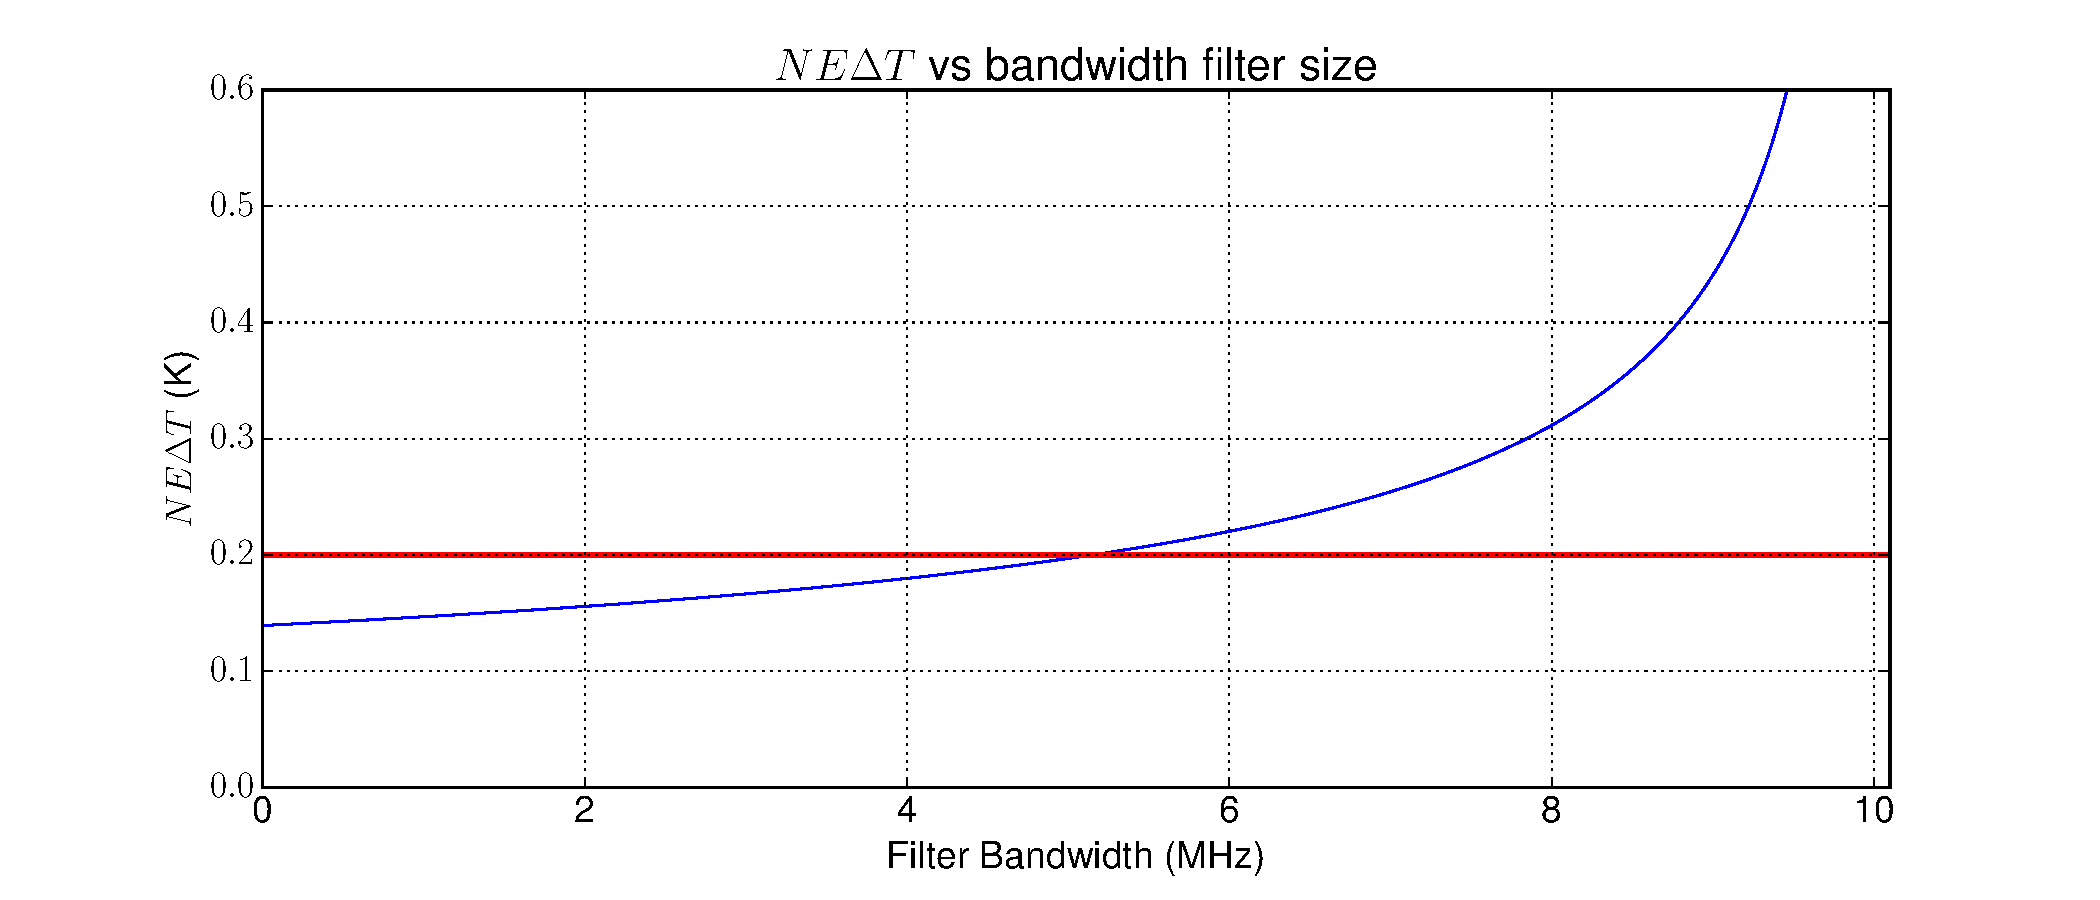
\includegraphics[width=\textwidth]{Experiments/Exp5/neatvsbw_plot.pdf}
\isucaption{Graph of the calculated $NE\Delta T$, the proposed limit for the sensitivity of the radiometer, and the measured standard deviation with repsect to filter bandwidth.}
\label{neat_bw}
\end{figure}

We can graph the expected response of the $NE\Delta T$ by adjusting the values of $\beta_{fitler}$ to range from a narrow-band filter, in our example 125 kHz, all the way to 9.99 MHz or nearly all of the bandwidth.  Figure \ref{neat_bw} shows the expected exponential response of $NE\Delta T$ as the size of the filter increases.  

Figure \ref{neat_bw} shows measured standard deviation points for the SDR-based radiometer for different filter sizes.  These filter sizes and collected data found is found in Table \ref{exp4_data_power}.  It can be seen in Figure \ref{neat_bw} that there is a good correlation between the expected sensitivity of the radiometer and the measured sensitivity of the radiometer.

\begin{figure}[h!tb] \centering
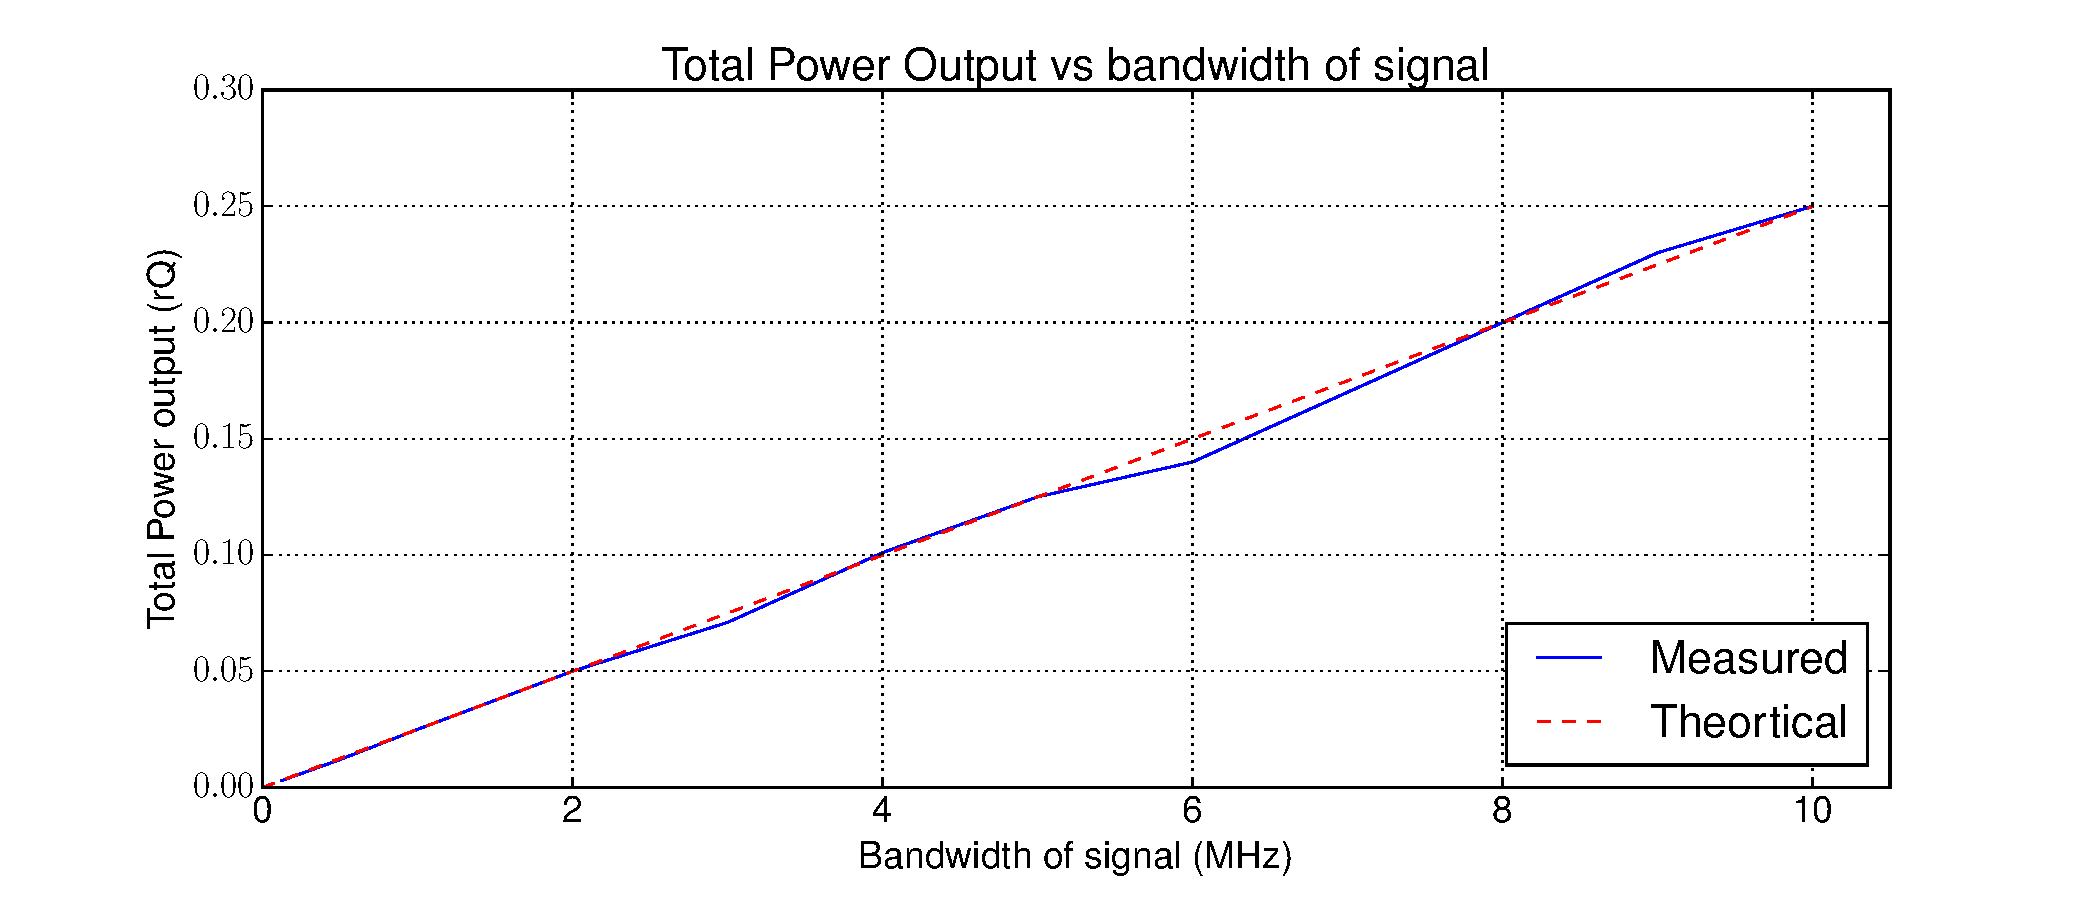
\includegraphics[width=\textwidth]{Experiments/Exp5/combined_plot.pdf}
\isucaption{Graph of the total power measured and theoretical power versus the bandwidth of the measured signal.}
\label{power_bw}
\end{figure}

Finally a line is added to Figure \ref{neat_bw} to show a possible limit of when we may have filtered too much.  In this example a $NE\Delta T$ of 0.2 Kelvin is used.  In Figure \ref{neat_bw} it can be seen that at about 5 MHz, our $NE\Delta T$ exceeds our threshold of 0.2 Kelvin.  This would mean that to meet this performance criteria we would need to not exceed 5 MHz for our filter size.  This is assuming our integration time ($\tau$) and the bandwidth ($\beta$) is held constant. 

We now look at the relationship of the total power received as the bandwidth decreases.  Figure \ref{power_bw} shows both the measured total power received and the expected total power received as the bandwidth of the filter increases.

The total power is calculated from Equation \ref{eq:final_power} and is based on the system noise ($T_N$), and the antenna ($T_A$), the bandwidth ($\beta$) and the gain ($G$) of the amplifiers used.  Our gain and noise temperatures are fixed, and in this experiment we use a system gain of 30 dB.  This represents the gain that we see with the three LNAs used minus any losses or attenuation placed in the RF chain.  What changes in this experiment is the amount of bandwidth.  Again, we can modify Equation \ref{eq:final_power} by subtracting the filter bandwidth ($\beta_{filter}$) from the total bandwidth available and is shown in Equation \ref{PWR_FILTER}.

\begin{equation}\label{PWR_FILTER}
P_{out}=k (\beta - \beta_{filter})G(T_{A}+T_{N})
\end{equation}

To compare this theoretical power to the actual power measured, we collected the rQ values by once again creating different filter sizes and then measuring the rQ values.  These values can be found in Table \ref{exp4_datapoints} and are added as dots to Figure \ref{power_bw}.  This also shows a very good correlation between the expected total power received and the measured total power received for Experiment IV.

\subsection{Usage Scenario}
%Move this section to 6.4.3 and edit
\emph{Application with Soil Moisture Readings}.  A common application of radiometers is in the measurement of soil moisture.  All items naturally emit RF energy due to the random excitation by the electrons in the object.  The amount of noise that gets generated varies by temperature and the amount that reaches the antenna varies by the amount of moisture in the soil.  If we calibrate the radiometer to two known soil conditions, then we can measure the various levels of soil moisture in the soil.  We will assume the soil is at a constant temperature during the observation.  We will look at the percentage of moisture in the soil, which will vary from zero percent or dry soil to one hundred percent or very wet soil.  The drier the soil, the more thermal noise we receive and the "warmer" the noise temperature.  Wet soil on the other hand attenuates the thermal noise and shows up as a "cooler" noise temperature.  

Using the SDR-based radiometer, we can configure it to observe a soil sample area.  Since we do not have an antenna hooked up, we will simulate this by using a matched load submerged in two reference temperatures.  We will use the ice water bath and LN2 bath that was used in previous experiments for our reference temperatures.

Figure \ref{SDR_soil} shows the data collected from Experiment I.  If we assume that our LN2 is dry soil and that our ice water bath is wet soil, we can now interpolate the data to this scale and show the information we obtained in Experiment one as both a noise temperature and soil moisture.

\begin{figure}[h!tb] \centering

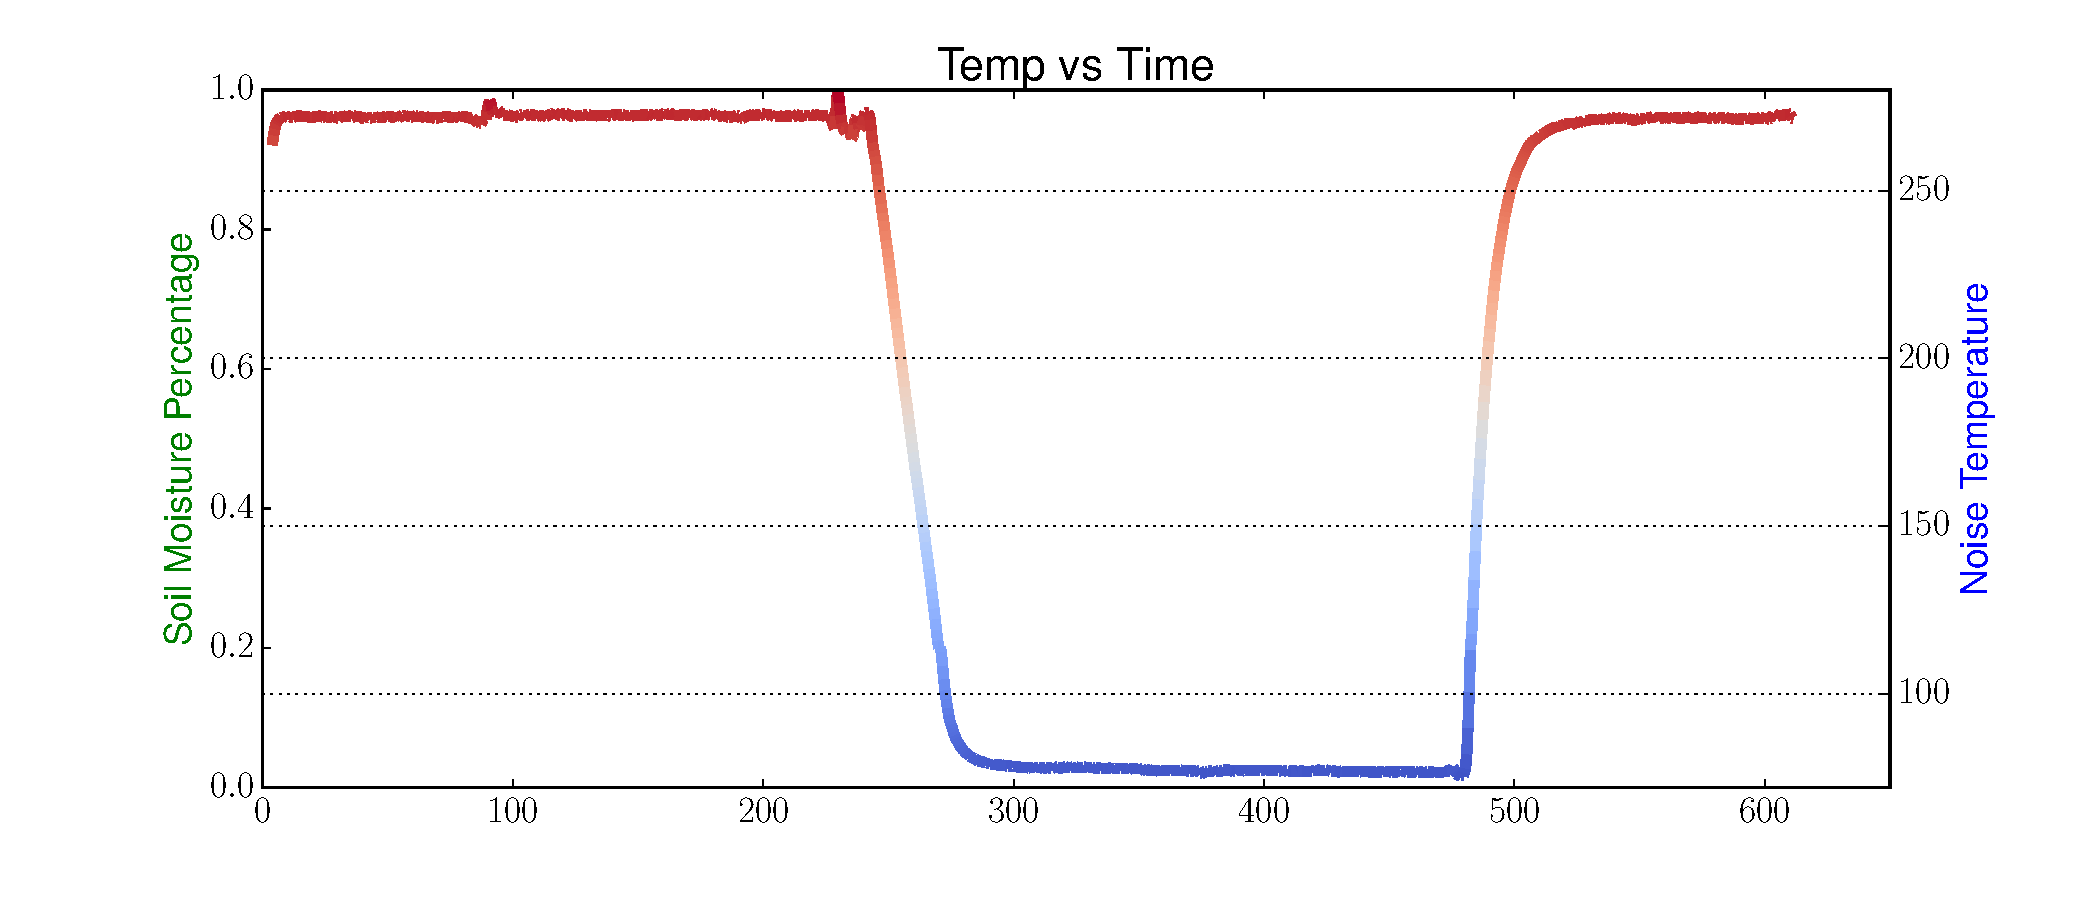
\includegraphics[width=\textwidth]{Experiments/Exp1/sdr_soilmoisture.pdf}
\isucaption{Plot of the noise temperature of Experiment I with soil moisture percentage added.}
\label{SDR_soil}
\end{figure}

While this demonstrates that we can calibrate our total power readings with a soil moisture percentage, we would use actual field tests to calibrate the radiometer.  In addition, we could also calibrate to soil moisture content instead of a percentage if desired.  Both methods have been done with traditional radiometers[\cite{Jonard}][\cite{Shi}.

\emph{Mitigating interference.} Experiment III demonstrates that an offending signal will impact and cause the total power received to increase.   This increase in total power will then invalidate our calibration of the SDR-based radiometer.  This will result in a spike as shown in Figure \ref{sdr_unfilt_raw}.  This spike shows a higher than normal total power which will result in a higher noise temperature.  A higher noise temperature will then cause the SDR-based radiometer to show drier soil conditions than what is actually present.

By mitigating the interfering signal the SDR-based radiometer is able to make calibrated soil moisture measurements even with the signal present.  Figure \ref{sdr_calib_filter} demonstrates the SDR-based radiometer making total power measurements with an offending signal present.  

Soil moisture measurements can continue with an offending signal present, however there is an impact on the system with filtering out this signal.  This is covered in Section \ref{Exp4_results}.  Because of this impact, re-calibration of the SDR-based radiometer still needs to take place.  Therefore while this solution is viable for interfering signals that are constant, other methods would need to be developed to handle sporadic interference.  

\emph{Example experiment.}  An example of how a SDR-based radiometer would mitigate a signal for a soil moisture reading is outlined next.  The SDR-based radiometer is configured to record both total power measurements and the in-phase and quadrature-phase (i.e. I and Q) data.  The recorded data is then analyzed after the experiment is over and it is observed that the total power readings have erratic readings.  Displaying the frequency and magnitude information that is generated from the I/Q data shows an interfering signal is present.  It can be determined from this information the frequency and magnitude the offending signal is located.  A band-reject filter is then designed to notch the offending signal out from the data.  The experiment can now be re-played with the filter active and new total power measurements are now recorded with out the offending signal.

As discussed in Section \ref{Exp4_results}, the performance of the radiometer will change depending on the bandwidth of the filter used for the signal.  Figure \ref{power_bw} however, shows that the relationship between the bandwidth of the signal and the total power received is a linear relationship and can therefore be predicted.  We can therefore compensate for the filter to maintain the calibration of the radiometer.

%---------------------------------------------------------------

\section{Advantages of a Software Defined Radio Based Radiometer}
A study was conducted on what benefits a software defined radio radiometer would have over a more traditional radiometer.  We focused on three main areas; cost, weight and size, and the value a SDR-based radiometer can add over traditional radiometers.

\subsection{Cost Benefits}
Software defined radios have become more commonplace in recent years and this has generated a number of Commercial Off The Shelf (COTS) solutions.  A COTS solution is often a lower cost solution due to the mass manufacturing that takes place.  This has driven the cost of many SDRs to under one thousand dollars, while still having excellent performance characteristics.  The N200 SDR purchased for this research cost fifteen hundred dollars and the daughter-board approximately cost one hundred and fifty dollars.  Other software defined radios however have come out on the market since then.  Ettus, for example, has some that are below one thousand dollars and the author has also obtained the HackRF One SDR that now sells for three hundred dollars.  The main difference between defined radios on the market is in their resolution and the bandwidth they support.

\begin{table}[h!tb] \centering
\isucaption{Cost Analysis}
\label{cost_table}
% Use: \begin{tabular{|lcc|} to put table in a box
\begin{tabular}{lcc} \hline
\textbf{Device} & \textbf{Quantity} & \textbf{Cost} \\ \hline
\textbf{SDR Solution}& & \\ \hline
N200 SDR & 1 & \$1515 \\
LNA at \$60 ea. & 3 & \$180 \\
DBSRX2 Daughter-board & 1 & \$152 \\
GNURadio & 1 & \$0 \\ \hline
Total & & \$1847 \\ \hline
\textbf{ISU Radiometer} \\ \hline
LNA, FPGA, ADC, Microcontroller and power supplies & 1 & \$10,000\tablefootnote{Purchase price in 2005} \\ \hline
\textbf{Commercial Off the Shelf Unit}\\ \hline
Spectracyber 1420 MHz Hydrogen Line Spectrometer & 1 & \$2,650 \\ \hline

\end{tabular}
\end{table}

As seen in Table \ref{cost_table}, even the higher cost Ettus research equipment is a lower cost option than the custom built radiometer in use at Iowa State University, and even a comparable off the shelf radiometer.  It should be noted that the radiometer in use at Iowa State University is also a dual polarization radiometer so there are two RF front ends and two ADCs that feed into a FPGA board.  It would be quite easy to add dual polarization to the Ettus N200 SDR as it does support two daughter-boards.  This would increase the cost to \$2,179 for the additional LNAs and daughter-board.

The largest cost benefit is that key components that you find in a radiometer, the filters and square-law detector, can be performed in software instead of needing additional equipment.  The system is also much more frequency agile, which means it can work over a broader range of frequencies than most traditional radiometers, with very little change in hardware and in some cases may require no change in hardware.  The Ettus N200, for example, uses daughter-boards to provide the RF interface.  While these boards provide a high quality RF signal, it does come at a cost and are usually designed for certain bands of frequencies.  Other low cost SDRs, however, also support a wide range of frequencies.  The HackRF, for example, works from 10 MHz to 6 GHz, but does so at the cost of lower resolution, less gain in its front-end, and supports a lower bandwidth.

\subsection{Weight and component size benefits}

A typical radiometer has many components that are involved in its design.  This includes filters, LNAs, and the power detection (i.e. square-law detector) used.  These components add weight, size and costs to a radiometer.  A software defined radio however digitizes the signal and we are able to replace the filters and square-law detector with their software equivalent.  While a software defined radio does add an ADC and usually a FPGA to perform signal processing, advances in semiconductor technology has continued to shrink these components.  These components are also lighter than the filters often used in traditional radiometers.  Table \ref{weight_table} displays the mass for the SDR-based radiometer built and the ISU Radiometer.  The ISU Radiometer is a representation of most traditional radiometers.

\begin{table}[h!tb] \centering
\isucaption{Weight Analysis}
\label{weight_table}
% Use: \begin{tabular{|lcc|} to put table in a box
\begin{tabular}{lc} \hline
\textbf{Device} & \textbf{Mass} \\ \hline
\textbf{SDR Solution} & \\ \hline
N200 SDR & 1.2 kg \\
LNA at .03 kg ea & .09 kg \\
DBSRX2 Daughter-board & .1 kg \\ \hline
Total & 1.39 kg \\ \hline
\textbf{ISU Radiometer} \\ \hline
LNA, FPGA, ADC, Microcontroller and power supplies & 22.7 kg \\ \hline
\textbf{Commercial Off the Shelf Unit}\\ \hline
Spectracyber 1420 MHz Hydrogen Line Spectrometer & 6 kg\tablefootnote{Estimated, no data available} \\ \hline

\end{tabular}
\end{table}

Size is another benefit, since semiconductor technology has continued to shrink components.  Again, since items like the filters and square-law detector are replaced with software implementations, this helps to reduce the overall size.  

\subsection{Value added benefits}

A SDR-based radiometer adds additional value for two reasons.  One, it is able to work with both frequency and magnitude information, where a traditional radiometer does not.  This allows for additional analysis on the signal and can help identify issues such as an interfering signal that was demonstrated in this thesis.  

Second, we are able to have an agile system that is able to adapt to changing conditions with very little or no change to hardware.  Different types of radiometers can be implemented such as a Dicke radiometer, dual polarization radiometer, or a radiometer that can perform Stokes parameters.  In addition, since we have both frequency and power information, we can create a system that is able to adapt to changing conditions, such as dealing with an interfering signal.  

\section{Drawbacks of a SDR-based Radiometer}
Although we have outlined a number of advantages of using a COTS SDR-based Radiometer and how a SDR can add additional value to the radiometer system, there are some disadvantages to a SDR-based Radiometer.

\subsection{Power Consumption}
One of the largest drawbacks to a SDR-based radiometer can be in the power consumption of the SDR.  With the move to perform functions such as power detection and filtering we now require additional computational power to perform these tasks.  With those computational cycles additional power is now required.  The use of FPGAs and SoC can help to minimize these power concerns as they are more efficient than using a PC.  

Power and CPU requirements also increase as we add additional functionality such as filtering an offending signal.  While these additions may not require additional hardware, it can require additional processor and memory requirements.  An increase and processing requirements will also increase power requirements and can also add additional requirements in cooling.

\subsection{Bandwidth constraints}
While SDR technology has advanced, bandwidth is still a constraint that affects SDRs and in turn a SDR-based Radiometer.  Bandwidth plays a critical role in a radiometer's sensitivity as explained in this thesis, therefore the fact that many SDRs are limited in bandwidth does create a disadvantage.  In many cases, this bottleneck takes place in both the transport and processing of large bandwidth systems.  This also relates to the power consumption disadvantage since larger bandwidth also means requiring additional computational cycles.

In contrast, a square-law detector usually has a very large bandwidth, as much as one gigahertz, and is why we usually need to filter to the frequency band of interest.  

%----------------------------------------------------------
% End of Chapter 6.  Anything below this is extra information

